\documentclass[times,specification,annotation]{itmo-student-thesis}

%% Опции пакета:
%% - specification - если есть, генерируется задание, иначе не генерируется
%% - annotation - если есть, генерируется аннотация, иначе не генерируется
%% - times - делает все шрифтом Times New Roman, собирается с помощью xelatex
%% - languages={...} - устанавливает перечень используемых языков. По умолчанию это {english,russian}.
%%                     Последний из языков определяет текст основного документа.

%% Делает запятую в формулах более интеллектуальной, например:
%% $1,5x$ будет читаться как полтора икса, а не один запятая пять иксов.
%% Однако если написать $1, 5x$, то все будет как прежде.
\usepackage{icomma}

%% Один из пакетов, позволяющий делать таблицы на всю ширину текста.
\usepackage{tabularx}

%% Данные пакеты необязательны к использованию в бакалаврских/магистерских
%% Они нужны для иллюстративных целей
%% Начало
\usepackage{tikz}
\usetikzlibrary{arrows}
\usepackage{filecontents}
\begin{filecontents}{bachelor-thesis.bib}
@inproceedings{cai2020understanding,
  title={Understanding and optimizing persistent memory allocation},
  author={Cai, Wentao and Wen, Haosen and Beadle, H Alan and Hedayati, Mohammad and Scott, Michael L},
  booktitle={Proceedings of the 25th ACM SIGPLAN Symposium on Principles and Practice of Parallel Programming},
  pages={421--422},
  year={2020},
  langid={english}
}

@article{denning1970virtual,
  title={Virtual memory},
  author={Denning, Peter J},
  journal={ACM Computing Surveys (CSUR)},
  volume={2},
  number={3},
  pages={153--189},
  year={1970},
  publisher={ACM New York, NY, USA},
  langid={english}
}

@online{thread-local-storage,
    year        = {2020},
    title       = {Thread-local storage},
    url         = {https://en.wikipedia.org/wiki/Thread-local_storage},
    langid      = {english}
}

@online{mmap,
    year        = {2020},
    title       = {mmap(2)},
    url         = {http://man7.org/linux/man-pages/man2/mmap.2.html},
    langid      = {english}
}

@online{msync,
    year        = {2020},
    title       = {msync(2)},
    url         = {http://man7.org/linux/man-pages/man2/msync.2.html},
    langid      = {english}
}

@online{kill,
    year        = {2020},
    title       = {kill(1)},
    url         = {https://man7.org/linux/man-pages/man1/kill.1.html},
    langid      = {english}
}


@online{compare-and-swap,
    year        = {2020},
    title       = {compare-and-swap},
    url         = {https://en.wikipedia.org/wiki/Compare-and-swap},
    langid      = {english}
}

@online{test-and-set,
    year        = {2020},
    title       = {test-and-set},
    url         = {https://en.wikipedia.org/wiki/Test-and-set},
    langid      = {english}
}

@online{fetch-and-add,
    year        = {2020},
    title       = {fetch-and-add},
    url         = {https://en.wikipedia.org/wiki/Fetch-and-add},
    langid      = {english}
}

@online{program-counter,
    year        = {2020},
    title       = {Program counter},
    url         = {https://en.wikipedia.org/wiki/Program_counter},
    langid      = {english}
}

@online{pipe,
    year        = {2020},
    title       = {pipe(2)},
    url         = {https://man7.org/linux/man-pages/man2/pipe.2.html},
    langid      = {english}
}

@online{posix-mq,
    year        = {2020},
    title       = {POSIX message queues},
    url         = {https://www.man7.org/linux/man-pages/man7/mq_overview.7.html},
    langid      = {english}
}

@online{file-locking,
    year        = {2020},
    title       = {File locking},
    url         = {https://en.wikipedia.org/wiki/File_locking},
    langid      = {english}
}

@online{posix-sems,
    year        = {2020},
    title       = {POSIX semaphores},
    url         = {https://man7.org/linux/man-pages/man7/sem_overview.7.html},
    langid      = {english}
}

@online{malloc,
    year        = {2020},
    title       = {malloc(3)},
    url         = {https://man7.org/linux/man-pages/man3/malloc.3.html},
    langid      = {english}
}

@online{calling-conventions,
    year        = {2020},
    title       = {x86 calling conventions},
    url         = {https://en.wikipedia.org/wiki/X86_calling_conventions},
    langid      = {english}
}

@online{hoare-monitor,
    year        = {2020},
    title       = {Monitor},
    url         = {https://en.wikipedia.org/wiki/Monitor_(synchronization)},
    langid      = {english}
}

@online{process,
    year        = {2020},
    title       = {Process},
    url         = {https://en.wikipedia.org/wiki/Process_(computing)},
    langid      = {english}
}

@online{gtest,
    year        = {2020},
    title       = {gtest},
    url         = {https://github.com/google/googletest},
    langid      = {english}
}

@online{thread,
    year        = {2020},
    title       = {Thread},
    url         = {https://en.wikipedia.org/wiki/Thread_(computing)},
    langid      = {english}
}

@online{pmdk,
    year        = {2020},
    title       = {PMDK},
    url         = {https://github.com/pmem/pmdk/},
    langid      = {english}
}



@inproceedings{attiya2018nesting,
  title={Nesting-safe recoverable linearizability: Modular constructions for non-volatile memory},
  author={Attiya, Hagit and Ben-Baruch, Ohad and Hendler, Danny},
  booktitle={Proceedings of the 2018 ACM Symposium on Principles of Distributed Computing},
  pages={7--16},
  year={2018},
  langid={english}
}

@article{friedman2018persistent,
  title={A persistent lock-free queue for non-volatile memory},
  author={Friedman, Michal and Herlihy, Maurice and Marathe, Virendra and Petrank, Erez},
  journal={ACM SIGPLAN Notices},
  volume={53},
  number={1},
  pages={28--40},
  year={2018},
  publisher={ACM New York, NY, USA},
  langid={english}
}

@book{ kerrisk,
    author      = {Michael Kerrisk},
    title       = {The Linux Programming interface},
    address     = {San Francisco},
    publisher   = {William Pollock},
    numpages    = {1552},
    pagetotal   = {1556},
    year        = {2010},
    langid      = {english}
}

@inproceedings{cai2020understanding,
  title={Understanding and optimizing persistent memory allocation},
  author={Cai, Wentao and Wen, Haosen and Beadle, H Alan and Hedayati, Mohammad and Scott, Michael L},
  booktitle={Proceedings of the 25th ACM SIGPLAN Symposium on Principles and Practice of Parallel Programming},
  pages={421--422},
  year={2020},
  langid={english}
}

@article{herlihy1990linearizability,
  title={Linearizability: A correctness condition for concurrent objects},
  author={Herlihy, Maurice P and Wing, Jeannette M},
  journal={ACM Transactions on Programming Languages and Systems (TOPLAS)},
  volume={12},
  number={3},
  pages={463--492},
  year={1990},
  publisher={ACM New York, NY, USA},
  langid={english}
}

@article{papadimitriou1979serializability,
  title={The serializability of concurrent database updates},
  author={Papadimitriou, Christos H},
  journal={Journal of the ACM (JACM)},
  volume={26},
  number={4},
  pages={631--653},
  year={1979},
  publisher={ACM New York, NY, USA},
  langid={english}
}

@incollection{lamport2019time,
  title={Time, clocks, and the ordering of events in a distributed system},
  author={Lamport, Leslie},
  booktitle={Concurrency: the Works of Leslie Lamport},
  pages={179--196},
  year={2019},
  langid={english}
}

@article{herlihy1991wait,
  title={Wait-free synchronization},
  author={Herlihy, Maurice},
  journal={ACM Transactions on Programming Languages and Systems (TOPLAS)},
  volume={13},
  number={1},
  pages={124--149},
  year={1991},
  publisher={ACM New York, NY, USA},
  langid={english}
}

@inproceedings{izraelevitz2016linearizability,
  title={Linearizability of persistent memory objects under a full-system-crash failure model},
  author={Izraelevitz, Joseph and Mendes, Hammurabi and Scott, Michael L},
  booktitle={International Symposium on Distributed Computing},
  pages={313--327},
  year={2016},
  organization={Springer},
  langid={english}
}


\end{filecontents}
%% Конец

\newcommand{\mynote}[3]{
    \fbox{\bfseries\sffamily\scriptsize#1}
{\small$\blacktriangleright$\textsf{\emph{\color{#3}{#2}}}$\blacktriangleleft$}}

\newcommand{\va}[1]{\mynote{Vitaly}{#1}{magenta}}
\newcommand{\ik}[1]{\mynote{Ilya}{#1}{green}}

\usepackage{graphicx}
\graphicspath{{pictures/}}

%% Указываем файл с библиографией.
\addbibresource{bachelor-thesis.bib}

\begin{document}


\studygroup{M3439}
\title{Исследование базовых алгоритмов и структур данных для non-volatile memory}
\author{Кокорин Илья Всеволодович}{Кокорин И.В.}
\supervisor{Аксёнов Виталий Евгеньевич}{Аксёнов В.Е.}{к.т.н.}{научный сотрудник ФИТиП}
\publishyear{2020}
%% Дата выдачи задания. Можно не указывать, тогда надо будет заполнить от руки.
\startdate{01}{сентября}{2019}


\secretary{Павлова О.Н.}

%% Задание
%%% Техническое задание и исходные данные к работе
\technicalspec{Требуется разработать алгоритм запуска программ для энергонезависимой байтоадресуемой памяти с произвольным доступом в модели Nesting-safe recoverable linearizability. Полученный алгоритм должен исполнять программы для энергонезависимой байтоадресуемой памяти и восстанавливать систему после сбоя. Кроме того, должна быть возможность эмулировать данный алгоритм и запускать программы для энергонезависимой байтоадресуемой памяти с произвольным доступом на системах, в которых в качестве энергонезависимого хранилища используются жёсткие диски.}

%%% Содержание выпускной квалификационной работы (перечень подлежащих разработке вопросов)
\plannedcontents{Необходимо изучить архитектуру энергонезависимой байтоадресуемой памяти с произвольным доступом и примеры алгоритмов для этой памяти, а также разработать алгоритм исполнения программ в этой памяти. После этого необходимо эмулировать разработанный алгоритм с помощью системы, использующей жёсткие диски в качестве энергонезависимого хранилища и протестировать с его помощью алгоритм CAS.}

%%% Исходные материалы и пособия 
\plannedsources{\begin{enumerate}
    \item Статья \cite{attiya2018nesting}
    \item Документация библиотеки \texttt{PMDK}
\end{enumerate}}

%%% Цель исследования
\researchaim{Разработать алгоритм исполнения программ в энергонезависимой памяти с произвольным доступом (NVRAM)}

%%% Задачи, решаемые в ВКР
\researchtargets{\begin{enumerate}
    \item Изучить архитекуру энергонезависимой памяти с произвольным доступом (NVRAM)
    \item Познакомиться с примерами конкурентных алгоритмов для NVRAM
    \item Разработать алгоритм исполнения конкуренных программ для NVRAM и восстановления системы после сбоя
    \item Эмулировать разработанный алгоритм с помощью системы, использующей жёсткие диски в качестве энергонезависимого хранилища
    \item Протестировать с его помощью изученный ранее алгоритм CAS для NVRAM
\end{enumerate}}

%%% Использование современных пакетов компьютерных программ и технологий
\addadvancedsoftware{Библиотека \texttt{PMDK} для работы с энергонезависимой памятью}{Реализация системы}
\addadvancedsoftware{Интегрированная среда разработки \texttt{CLion}}{Реализация системы}
\addadvancedsoftware{Распределённая система контроля версия \texttt{git}}{Реализация системы}
\addadvancedsoftware{Компилятор \texttt{GNU C++} языка \texttt{C++}}{Реализация системы}


%%% Краткая характеристика полученных результатов 
\researchsummary{Удалось разработать алгоритм запуска программ для NVRAM, который можно использовать как для запуска программ в системе с использованием NVRAM, так и в системе с использованием жёстких дисков в качестве энергонезависимого хранилища. Разработанный алгоритм был эмулирован на жёстких дисках с использованием библиотеки PMDK.}

%%% Гранты, полученные при выполнении работы 
\researchfunding{Грантов при выполнении работы получено не было.}

%%% Наличие публикаций и выступлений на конференциях по теме выпускной работы
\researchpublications{Победа в конкурсе докладов IX Конгресса Молодых Учёных}

%% Эта команда генерирует титульный лист и аннотацию.
\maketitle{Бакалавр}

%% Оглавление
\tableofcontents

\startrelatedwork
%% Макрос для введения. Совместим со старым стилевиком.
\startprefacepage

Целью работы была разработка алгоритма исполнения программ в энергонезависимой памяти с произвольным доступом (далее NVRAM).

\bigbreak

Передо мной стояли следующие задачи:

\begin{itemize}
    \item Изучить архитекуру энергонезависимой памяти с произвольным доступом (NVRAM).
    \item Познакомиться с примерами конкурентных алгоритмов для NVRAM.
    \item Разработать алгоритм исполнения конкурентных программ для NVRAM и для восстановления системы после сбоя.
    \item Проэмулировать разработанный алгоритм с помощью системы, использующей жёсткие диски в качестве энергонезависимого хранилища.
    \item Протестировать с его помощью изученный ранее алгоритм CAS для NVRAM.
\end{itemize}

\bigbreak

Актуальность задачи обусловлена существованием нескольких конкурентных алгоритмов для NVRAM, но отсутствием алгоритма их запуска и восстановления системы после сбоя. Это делает невозможным запуск и тестирование алгоритмов для NVRAM на реальных системах.

\bigbreak

Новизна работы обусловлена тем, что современные теоретические модели не учитывают архитектуру реальных систем. Например, подразумеватся отсутствие энергозависимых кэшей и регистров и наличие энергнезависимого стека, который мог бы сохранять состояние системы даже если в системе произошёл сбой. Например, в работе \cite{attiya2018nesting} подразумевается отсутствие кэшей и наличие энергонезависимого стека.

Поэтому новизна работы состоит в разработке алгоритма запуска программ для NVRAM на реальном железе с учётом всех его особенностей.

\bigbreak

Практическая значимость работы обусловлена тем, что представленное сегодня на рынке железо с NVRAM очень дорогое. Несмотря на это, существует потребность в тестировании алгоритмов для NVRAM. Если удастся эмулировать алгоритм запуска программ для NVRAM на более дешёвом железе (например, на жёстких дисках), это позволит тестировать алгоритмы для NVRAM даже без доступа к дорогому железу.

\bigbreak

Работа имеет следующую структуру:

\begin{itemize}
    \item В первой главе работы проводится анализ предметной области: рассматривается архитектура NVRAM, модели исполнения программ в системе с разделяемой энергонезависимой памятью, модели сбоев в такой системе и условия корректности исполнений в такой модели.
    
    \item Во второй главе разрабатывается алгоритм запуска программ на системе с NVRAM и восстановления системы после сбоя. Кроме того, рассматриваются вопросы: 1)~корректной работы с адресами функций и указателями на NVRAM, 2)~возврата значений из функций, запуска разработанного алгоритма на системе, использующей жёсткие диски в качестве энергонезависимого хранилища, и 3)~использования разработанного алгоритма для запуска программ, удовлетворяющих различным условиям корректности, например, линеаризуемости.

    \item В третьей главе рассматривается задача выделения памяти в куче NVRAM и представляются два достаточно простых алгоритма выделения памяти. Рассматриваются плюсы и минусы каждого из них, производится выбор подходящего нам алгоритма выделения памяти в куче NVRAM.
    
    \item В четвёртой главе рассматривается применение разработанного в предыдущих главах решения для запуска и тестирования на корректность алгоритма CAS для NVRAM, описанного в статье \cite{attiya2018nesting}. 
\end{itemize}

%% Начало содержательной части.
\chapter{Обзор предметной области}

\section{Архитектура NVRAM}

Архитектура NVRAM имеет следующие отличительные особенности:

\begin{itemize}
    \item Энергонезависимость, как у жёстких дисков. Это значит, что записанная в ней информация остаётся доступной даже в случае сбоя системы, и эту информацию можно использовать для восстановления системы после сбоя.
    
    \item Быстрый произвольный доступ с побайтовой адресацией, подобно оперативной памяти. Это позволяет придумывать для систем с NVRAM потенциально более эффективные алгоритмы восстановления системы после сбоя, чем традиционные алгоритмы на основе append-only журналирования, используемые на системах с жёсткими дисками. Для систем с жёсткими дисками такие алгоритмы, вероятно, будут неприменимы из-за низкой скорости случайного доступа, прямо вытекающей из механической природы жёстких дисков, но системы с NVRAM обеспечивают гораздо более быстрый случайный доступ и, следовательно, не имеют таких ограничений.
    
    \item Наличие в системе с NVRAM энергозависимой памяти. Например, кэши NVRAM и регистры всегда остаются энергозависимыми, вследствие чего при сбое системы теряются результаты последних вычислений (которые на x86 велись в регистрах) и данные, которые должны были быть записаны в NVRAM, но не успели записаться и попали в кэш. Для борьбы с потерей кэшированных данных системы с NVRAM предоставляют возможность явно потребовать сброса кэшей NVRAM в энергонезависимую память.
    
    \item Сброс данных в NVRAM производится кэш-линиями, при этом запись одной кэш-линии атомарна, то есть в случае сбоя в процессе записи вся кэш-линия либо целиком записывается, либо целиком не записывается в NVRAM. Запись, например, половины кэш-линии невозможна. Однако  запись большого количества данных, не влезающих в одну кэш линию, происходит неатомарно, так как сбой может произойти после записи первой кэш-линии, но до записи всех остальных. В таком случае первая кэш-линия будет записана в NVRAM, а остальные данные не будут записаны.
\end{itemize}

\section{Модель исполнения}

В этой секции будет описана модель исполнения в системе с общей памятью, которую я буду использовать в работе. Эта модель является дополненной версией модели, описанной в статье \cite{attiya2018nesting}.

В системе существует $n$ процессов $\{p_i\}_{i=1}^n$, исполняющихся одновременно и асинхронно, и $m$ расположенных в общей энергонезависимой памяти объектов $\{O_j\}_{j=1}^m$. Процессы взаимодействуют друг с другом, вызывая различные операции на объектах в общей памяти (см. Рисунок~\ref{model-shared-pic}).

\begin{figure}[H]
  \centering
  \caption{Процессы и общие объекты}
  \label{model-shared-pic}
  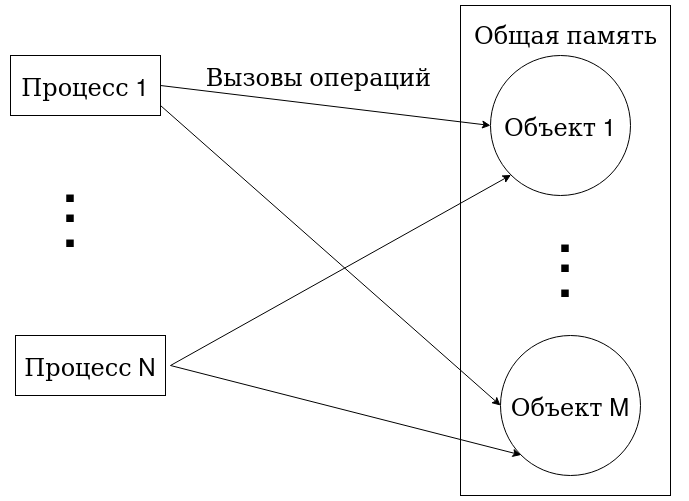
\includegraphics[width=\linewidth]{model_shared.png}
\end{figure}

Расположенные в общей памяти объекты могут поддержживать операции чтения (R), записи (W) и чтения-модификации-записи (RMW). 

Операцией чтения-модификации-записи (RMW) называется операция, которая атомарно исполняет следующие операции:
\begin{itemize}
    \item Читает записанное в ячейке памяти значение.
    
    \item Изменяет его неким образом (например, увеличивая на один).
    
    \item Записывает значение, полученное после изменения, обратно в ячейку памяти.
\end{itemize}

\bigbreak

Примерами таких операций являются \texttt{compare-and-swap} \cite{compare-and-swap}, \texttt{fetch-and-add} \cite{fetch-and-add}, \texttt{test-and-set} \cite{test-and-set}.

В работе \cite{herlihy1991wait} описано определение RMW-операции, примеры различных RMW-операций и их классификация.

В рассматриваемой модели вся разделяемая память является энергонезависимой, но подразумевается существование в системе также и энергозависимой памяти. Каждая ячейка энергозависимой памяти $reg_j$ является локальной для какого-то процесса $p_i$, это означает, что доступ к $reg_j$ может получать только процесс $p_i$ и ни один процесс, кроме $p_i$.

Таким образом, помимо доступа к разделяемым объектам, каждый процесс имеет доступ к локальным объектам, доступным только ему и недоступным другим процессам. Эти объекты хранятся в энергозависимой памяти данного процесса и поддерживают операции чтения (R) и записи (W) (см. Рисунок~\ref{model-local-pic}). 

\begin{figure}[H]
  \centering
  \caption{Процессы и локальные объекты}
  \label{model-local-pic}
  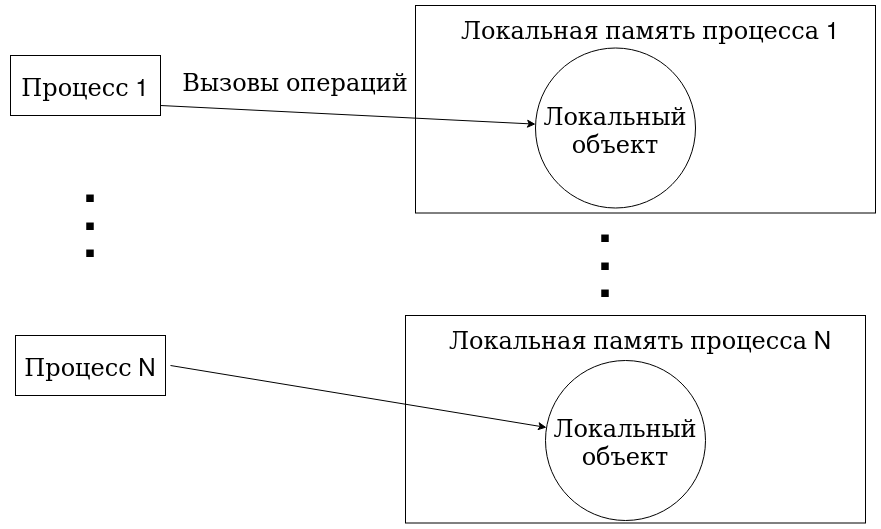
\includegraphics[width=\linewidth]{model_local.png}
\end{figure}

\bigbreak

При этом нам не важно, где именно расположены локальные объекты: в регистрах процессора, на стеке или в динамической памяти. Нас интересует только то, что все локальные объекты:

\begin{itemize}
    \item Расположены в энергозависимой памяти (а значит, их значение теряется при сбое системы - более подробно это свойство локальный объектов будет обсуждаться в секции \ref{crush-models}).
    
    \item Доступны только одному процессу.
\end{itemize}

\bigbreak

Рассмотренная модель не учитывает некоторые особенности реального железа: например, в ней не учитывается наличие энергозависимых кэшей NVRAM и возможность наличия в системе разделяемой энергозависимой памяти.

\section{Модели сбоев}
\label{crush-models}

Существуют две модели сбоев в системе.

\begin{itemize}
    \item Individual crash-failure.
    
    Эта модель описана в работе \cite{attiya2018nesting}. В такой модели каждый процесс может может столкнуться со сбоем в процессе работы независимо от остальных процессов системы. При сбое процесс перестаёт работать до тех пор, пока он не будет перезапущен. Перезапуск процесса восстанавливает его работоспособность, но при этом теряется значение всех локальных переменных, расположенных в энергозависимой памяти перезапускаемого процесса.
    
    Записанные же в NVRAM данные общих объектов не теряются и остаются доступными процессу после восстановления работы.

    Так как сбойный процесс неотличим от очень медленного, система при сбоях сохраняет гарантии прогресса, которым она удовлетворяла до сбоя. Например, lock-free алгоритм остаётся таковым, даже если один или несколько процессов системы столкнулись со сбоем в ходе работы.
    
    \item System crash-failure. 
    
    В этой модели сбой происходит не в одном процессе, а во всей системе сразу. Система перестаёт работать до тех пор, пока она не будет перезапущена целиком. При этом после восстановления каждый процесс системы теряет данные, записанные в его локальной энергозависимой памяти. Следовательно, в такой модели при сбое системы теряются все данные, записанные в энергозависимой памяти.
    
    Как и в предыдущей модели, после сбоя системы данные общих объектов, записанные в NVRAM, не исчезают при сбое, и после возобновления работы эти данные продолжают быть доступны всем процессам системы. После возобновления работы эти данные могут быть использованы для восстановления после сбоя. 
\end{itemize}

\bigbreak

Заметим, что модель System crash-failure является частным случаем модели Individual crash-failure, так как сбой всей системы может быть представлен как одновременный сбой каждого из $n$ индивидуальных процессов $\{p_i\}_{i = 1}^n$.

Несмотря на то, что модель Individual crash-failure является более общей моделью, в работе будем рассматривать модель System crash-failure, так как она более точно описывает процесс и последствия сбоя реальной системы. В реальной системе сложно себе представить ситуацию, при которой сбой происходит в одном процессе, но легко представить себе ситуацию, при которой сбой происходит во всех процессах сразу~--- это происходит, например, при выключении питания. Кроме того, на реальных системах проэмулировать сбой в модели System crash-failure гораздо проще.

\section{Исполнение операций}

Модель конкуррентного исполнения операций в NVRAM описана в статье \cite{attiya2018nesting}.

Каждой операции \texttt{Op}, которая может быть исполнена в системе, сопоставлена операция \texttt{Op.Recover}.  \texttt{Op.Recover} получает при вызове те же аргументы, что и \texttt{Op} и исполняется на том же объекте, что и \texttt{Op}. \texttt{Op.Recover} должна завершить операцию \texttt{Op} в случае, если в процессе исполнения \texttt{Op} произойдёт сбой системы.

Исполнением системы $H$ называется последовательность шагов $\{step\}_{i = 1}^Z$, при этом каждый шаг $step_i$ имеет один из четырёх следующих типов:

\begin{itemize}
    \item \texttt{INV(p, O, Op, args)}~--- вызов процессом \texttt{p} операции \texttt{Op} на объекте \texttt{O} с аргументами \texttt{args}
    
    \item \texttt{RES(p, O, Op, ret)}~--- завершение операции \texttt{Op}, вызванной на объекте \texttt{O} процессом \texttt{p}, результатом операции является \texttt{ret}.
    
    \item \texttt{CRASH}~--- сбой системы
    
    \item \texttt{RECOVER}~--- восстановление системы после сбоя.
\end{itemize}

\bigbreak

Операция \texttt{Op} называется исполняющейся на процессе \texttt{p}, если в этом процессе уже произошёл вызов этой операции, но ещё не произошёл возврат из неё. У процесса \texttt{p} в каждый момент может быть несколько исполняющихся операций одновременно (это происходит, например, если в ходе исполнения операции \texttt{F} происходит вызов операции \texttt{G}). В таком случае в каждом процессе исполняющиеся операции формируют вложенную последовательность (например, для примера выше будем говорить, что исполнение операции \texttt{G} вложено в исполнение операции \texttt{F}) (см. Рисунок~\ref{code-execution-pic}). 

\begin{figure}[H]
  \centering
  \caption{В момент  времени T на процессе p одновременно исполняются операции F и G, причём исполнение G вложено в исполнение F}
  \label{code-execution-pic}
  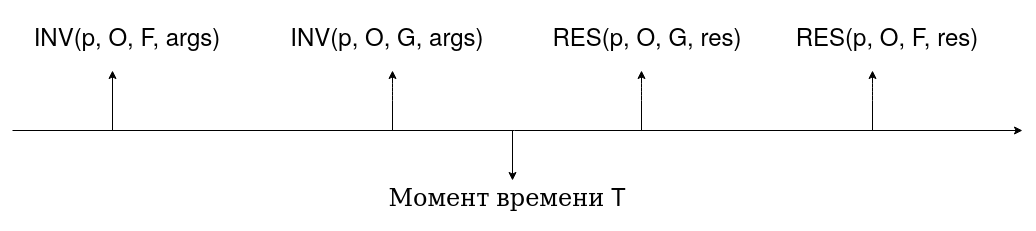
\includegraphics[width=\linewidth]{code_execution.png}
\end{figure}

Для восстановления системы после сбоя нужно для каждого процесса системы \texttt{p} вызвать \texttt{recover}-версию каждой операции, исполнявшейся в этом процессе в момент сбоя, начиная с той операции, которая была вызвана последней и заканчивая той, которая была вызвана первой. Например, в примере выше сначала будет вызвана операция \texttt{G.Recover}, а после её завершения \texttt{F.Recover} (см. Рисунок~\ref{code-execution-recovery-pic}).

\begin{figure}[H]
  \centering
  \caption{Восстановление системы после сбоя}
  \label{code-execution-recovery-pic}
  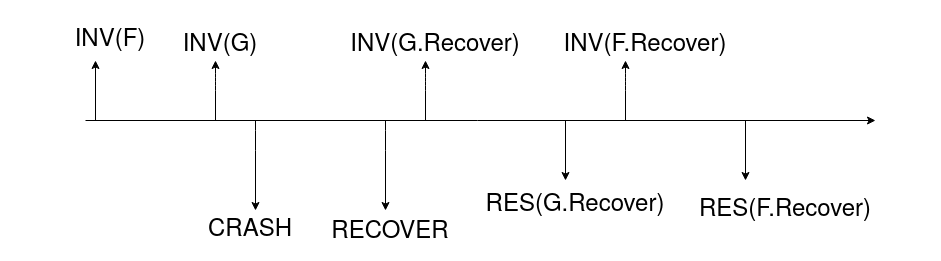
\includegraphics[width=\linewidth]{code_execution_recover.png}
\end{figure}

\section{Условия корректности}

Существует несколько условий корректности конкурентных алгоритмов для NVRAM. Перечислим их в порядке убывания строгости.

\begin{itemize}
    \item Nesting-safe recoverable linearizability описано в статье \cite{attiya2018nesting}. Это условие корректности требует, чтобы любая операция в системе была завершена даже в том случае, если в системе произошёл сбой. Для завершения операций, которые исполнялись в момент сбоя необходимо после восстановления запускать recover-версии операций, исполнявшихся в момент сбоя.
    
    \item Durable linearizability описано в статье \cite{izraelevitz2016linearizability}. Это условие корректности требует, чтобы эффект всех операции, исполнение которых завершилось до сбоя, был виден после восстановления. Если же операция исполялась в момент сбоя, то её эффект может быть как виден после восстановления, так и не виден.
    
    \item Buffered durable linearizability является ослабленной версией durable linearizability и описано в статье \cite{friedman2018persistent}. Это условие корректности отличается от последнего тем, что не требует после восстановления видимости эффектов всех операций, исполнение которых завершилось до сбоя. Это условие корректности допускает, что эффект только части таких операций будет виден после восстановления. Однако, это условие корректности требует, чтобы каждый объект предоставлял операцию \texttt{sync}. Если на объекте была вызвана операция \texttt{sync} и её исполнение завершилось до сбоя, то после восстановления должны быть видимы результаты всех операций, исполнение которых завершилось до вызова операции \texttt{sync}.
    
\end{itemize}

\bigbreak

В этой работе мы предоставляем алгоритм запуска программ, удовлетворяющих условиям Nesting-safe recoverable linearizability. 

\section{Описание существующих решений поставленной проблемы}

На текущий момент не существует алгоритмов запуска программ на системах с NVRAM, которые можно было бы эмулировать на системах, использующих жёсткие диски в качестве энергонезависимого хранилища, и использовать для тестирования алгоритмов для NVRAM даже без доступа к железу с NVRAM.

\chapterconclusion

В этой главе был проведён анализ предметной области: рассмотрена архитектура NVRAM, модели исполнения в системе с разделяемой энергонезависимой памятью, модели сбоев в такой системе, а также условия корректности таких исполнений. Кроме того, было определено понятие \texttt{recover}-операции, которое играет важную роль в следующих главах. Был проведён анализ существующих решений и показано, что разработанное решение является единственным в своём роде.

\finishrelatedwork

\chapter{Разработка системы исполнения и восстановления}
\label{system-impl}

\section{Процессы и потоки}

В теории конкуррентного программирования зачастую термины ``процесс'' и ``поток'' не различают и считают синонимами. Однако, при реализации алгоритмов очень важно понимать разницу между процессами и потоками, поэтому в дальнейшем будем их различать.

Будем использовать терминологию операционной системы Linux и считать, что каждый процесс \cite{process}

\begin{itemize}
    \item исполняется в собственном адресном пространстве;
    
    \item имеет иллюзию монопольного использования всей памяти системы (такая иллюзия достигается при помощи использования механизма виртуальной памяти, как это, например, описано в статье \cite{denning1970virtual});
    
    \item состоит из нескольких потоков.
\end{itemize}

\bigbreak

Все потоки \cite{thread} одного процесса разделяют единое адресное пространство этого процесса и, следовательно, имеют общую кучу и общую статическую память. Например, из этого следует, что все потоки одного процесса разделяют единый сегмент кода. Но каждый поток системы:

\begin{itemize}
    \item имеет собственное процессорное время;
    
    \item имеет собственный стек;
    
    \item имеет иллюзию монопольного использования регистров процессора~--- например, наличие у каждого потока независимого от остальных потоков регистра \texttt{RIP} позволяет всем потокам независимо исполнять код из сегмента кода процесса, поскольку каждый поток имеет собственный указатель на текущую исполняемую в потоке инструкцию \cite{program-counter}.

\end{itemize}

\bigbreak

Несмотря на то, что в большинстве случаев мы считаем, что все потоки одного процесса разделяют общую память, а различные процессы не разделяют память вообще, из этого правила бывают исключения. Потоки могут использовать thread-local storage \cite{thread-local-storage} для хранения статических данных, не разделяемых между потоками одного процесса, а доступных только одному потоку. Процессы же могут разделять память с другими процессами с использованием различных механизмов межпроцессного взаимодействия, например shared memory mapped files \cite{mmap}.

Использование процессов и потоков в операционной системе Linux описано, например, в книге \cite{kerrisk}.

Заметим, что сущности, называемые на практике (и, следовательно, в дальнейшем тексте) ``потоками'' соответствуют сущностям, называемым в теории конкуррентного программирования (и, следовательно, в первой главе) ``процессами''.

\section{Взаимодействие с NVRAM}

Считаем, что NVRAM предоставляет нам следующие функции:

\begin{itemize}
    \item \texttt{void pmem\_read(const void* src, void* dest, size\_t len)} копирует \texttt{len} байт из \texttt{src} (этот указатель должен указывать на участок NVRAM) в \texttt{dest} (этот указатель должен указывать на участок энергозависимой памяти) и, тем самым, позволяет читать данные из NVRAM в энергозависимую память.
    
    \item \texttt{void pmem\_write(void* dest, const void* src, size\_t len)} копирует \texttt{len} байт из \texttt{src} (этот указатель должен указывать на участок энергозависимой памятм) в \texttt{dest} (этот указатель должен указывать на участок NVRAM) и, тем самым, позволяет писать данные из энергозависимой памяти в NVRAM. Заметим, что данные после записи могут не попасть в NVRAM непосредственно, а остаться в кэше.
    
    \item \texttt{void pmem\_flush(const void* dest, size\_t len)} производит сброс энергозависимых кэшей в NVRAM, начиная с адреса \texttt{dest}. При этом сброшено будет не менее \texttt{len} байт. Следовательно, после завершения этого вызова все изменения, сделанные на интервале $[dest; dest + len)$ будут сброшены в NVRAM из кэша. При этом В NVRAM может быть сброшено более \texttt{len} байт, так как сброс данных в NVRAM производится кэш-линиями.  Например, невозможно произвести сброс одного байта в NVRAM, необходимо сбросить всю кэш-линию, в которой находится этот байт. После завершения вызова в NVRAM из кэша будут сброшен интервал $[left; right)$, при этом $[dest; dest + len) \subseteq [left; right)$, где $left$ - адрес начала кэш-линии. 
    
\end{itemize}

\section{Персистентный стек}
\label{persistent-stack}

Заметим, что для запуска программ на NVRAM, необходимо поддерживать информацию о том, какие операции исполнялись в момент сбоя в каждом потоке. Кроме того, необходимо поддерживать информацию о порядке их вызова для того, чтобы знать, в каком порядке запускать recover-операции.

Для того, чтобы поддерживать информацию о порядке вызова исполнявшихся в момент сбоя функций, необходимо просто для каждого потока поддерживать его стек, состоящий из стековых фреймов, по одному на каждую вызванную функцию. При вызове функции мы добавляем новый фрейм на вершину стека, при возврате из функции стираем последний стековый фрейм с вершины стека. Таким образом, в момент сбоя на стеке потока $t_i$ оказываются расположены стековые фреймы тех и только тех функций, которые исполнялись на этом потоке в момент сбоя. Причём, чем ближе стековый фрейм, соответствующий некой функции, расположен к вершине стека, тем позже в потоке была вызвана эта функция (см. Рисунок~\ref{execution-and-stack-pic}).

\begin{figure}[H]
  \centering
  \caption{Исполнение и соответствующий этому исполнению стек потока p}
  \label{execution-and-stack-pic}
  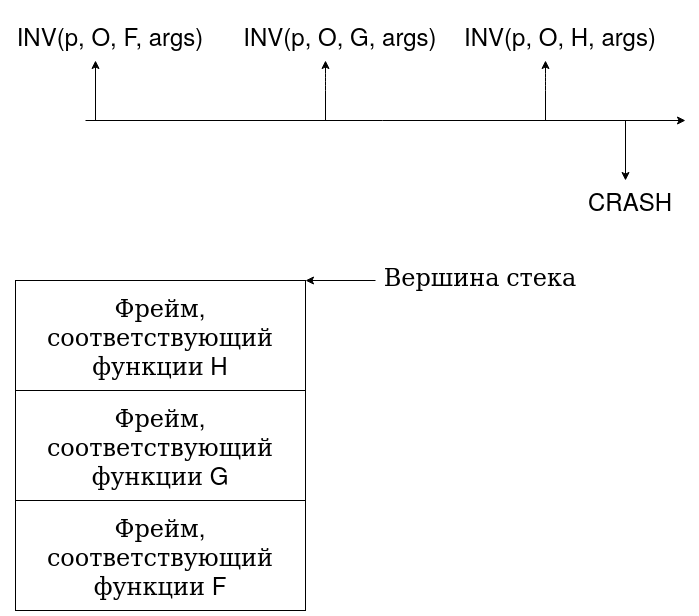
\includegraphics[width=\linewidth]{execution_and_stack.png}
\end{figure}

Для каждого потока операционная система итак поддерживает собственный стек вызовов. Проблема состоит в том, что стек вызовов выделяется в энергозависимой области памяти, а простой его перенос в энергонезависимую память проблему не решает.

Рассмотрим, например, передачу адресов возврата через стек вызовов. Если функция \texttt{f()} хочет вызвать функцию \texttt{g()}, вызывающая функция пишет на стек содержимое регистра \texttt{RIP} (указывающего на адрес команды, следующей за исполняющейся в текущий момент, то есть на адрес команды, следующей за командой \texttt{CALL g}) и передаёт управление вызываемой функции. Вызываемая функция, завершив работу, снимает со стека записанное там значение \texttt{RIP} и делает \texttt{JMP} на этот адрес чтобы вернуть управление коду вызывающей функции. Таким образом, после завершения этого перехода управление вернётся в вызывающую функцию на команду, следующую за командой \texttt{CALL g}.

Заметим, что если произойдёт сбой системы, а после повторного запуска системы мы перезапустим программу, операционная система заново выделит процессу память, в которую будет загружен код этого процесса. При этом операционная система может загрузить код процесса в другое место виртуальной памяти, т.е. не по тем же самым адресам, где код был расположен до сбоя. По этой причине записанные в стеке адреса возврата будут бессмысленны: память, на которую они указывают, может больше не содержать кода вообще. В лучшем случае это будет просто недоступная для чтения память, а в худшем случае она будет содержать произвольные данные, исполнение которых как кода вызовёт произвольные ошибки в ходе исполнения.

Следовательно, расположенные на стеке адреса возврата не могут помочь нам понять после возобновления работы системы, какие функции исполнялись в момент сбоя.

Для восстановления после сбоя критически необходимо знать, какие функции исполнялись в момент сбоя. И, так как стек операционной системы не может, по описанным выше причинам, предоставлять необходимую для восстановления информацию, будем поддерживать персистетный стек самостоятельно.

Для каждого потока, имеющего доступ к NVRAM, будем поддерживать персистентный стек особым образом.

Персистентный стек доступен только одному потоку и выделяется до создания этого потока. Стек имеет константный размер и не перевыделяется при переполнении. Всё это делает персистентный стек очень похожим на обычный стек операционной системы. Отличие состоит, во-первых, в том, что персистентный стек хранится в NVRAM, а во-вторых, в том, как этот стек поддерживается.

Персистентный стек состоит из персистентных стековых фреймов~--- по одному фрейму на каждую функцию, в которой происходит доступ к NVRAM (на чтение или запись). Каждая такая функция должна иметь \texttt{recover}-версию, которая получает те же аргументы, что и исходная функция, и должна завершить операцию в случае, если во время её исполнения или исполнения исходной функции произойдёт сбой.

Функции, в коде которых не происходит доступа к NVRAM, а происходит доступ только к локальным данным потока, хранящимся в энергозависимой памяти, не важны для алгоритма. Исполнение этих функций никак не меняет NVRAM, после сбоя результаты их запуска и частичного исполнения не будут видимы. Поэтому для таких функций не нужны \texttt{recover}-версии и при вызове таких функций мы не будем создавать персистентные стековые фреймы. Не умаляя общности, можно считать, что тела таких функций подставляются на место их вызова.

Каждый фрейм, кроме последнего, завершается однобайтным маркером конца фрейма (этот маркер имеет вид \texttt{0х0}). Последний фрейм завершается однобайтным маркером конца стека (этот маркер имеет вид \texttt{0х1}). После конца стека могут идти произвольные данные, эти данные никогда не нужно читать и интерпретировать (см. Рисунок~\ref{stack-structure-pic}).

\begin{figure}[H]
  \centering
  \caption{Структура персистентного стека}
  \label{stack-structure-pic}
  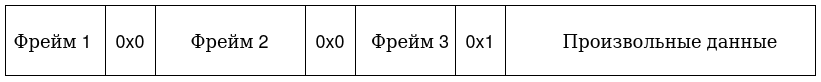
\includegraphics[width=\linewidth]{1.png}
\end{figure}

\section{Персистентный стековый фрейм}

Каждый персистентный стековый фрейм соответствует вызову некой функции \texttt{Op}. Фрейм содержит информацию, которая поможет при возобновлении работы системы определить адреса \texttt{Op} и \texttt{Op.Recover}, размер аргументов функции в байтах, сами аргументы, сериализованные в массив байт, место под ответ и в последнем байте фрейма маркер конца фрейма или маркер конца стека.

По причинам, объяснённым в секции \ref{persistent-stack}, в персистентном фрейме нельзя хранить адреса \texttt{Op} и \texttt{Op.Recover}.

Для решения этой проблемы можно хранить на стеке не адрес функции, а её  уникальный идентификатор, который, в отличие от адреса функции, не будет меняться от запуска к запуску. Например, в качестве идентификатора функции можно использовать имя этой функции (в таком случае требуется чтобы в системе не сущестовало двух функций с одинаковым именем).

В таком случае нужно уметь сопоставлять идентификатору функции адрес самой функции и её \texttt{recover}-версии. Для решения этой проблемы можно хранить в системе глобальную хеш-таблицу, сопоставляющую имени функции два адреса~--- самой функции и её \texttt{recover}-версии. В таком случае при каждом запуске системы необходимо заполнить эту хеш-таблицу, занеся в неё имена и адреса всех имеющих доступ к NVRAM функций, которые будут использоваться в ходе работы. Эта хеш-таблица должна храниться в энергозависимой памяти и заполняться каждый раз при перезапуске процесса, так как с каждым новым стартом системы код функций может менять своё расположение в памяти.

Так как для восстановления системы после сбоя необходимо выполнить \texttt{recover}-версии всех операций, которые исполнялись в момент сбоя, на стеке необходимо помимо идентификатора функции (чтобы знать, какую конкретно функцию исполнять) сохранять и её аргументы (чтобы знать, какие аргументы передавать \texttt{recover}-функции при запуске).

Будем хранить фреймы на стеке так, чтобы начало каждого фрейма было выровнено по размеру кэш-линии на используемой архитектуре. Смысл этого принципа станет понятен в секции \ref{return-value-stack}.

Будем хранить на стеке фреймы со следующей структурой (см. Рисунок~\ref{frame-structure-pic}):

\begin{itemize}
    \item $0 \leq n < \texttt{CACHE\_LINE\_SIZE}$ (где \texttt{CACHE\_LINE\_SIZE} это размер кэш-линии на данной архитектуре в байтах) неиспользуемых байт. Это поле не содержит никакой полезной информации и предназначено для того, чтобы адрес начала фрейма был кратен \texttt{CACHE\_LINE\_SIZE}. 
    
    \item Поле для возврата ответа. Размер этого поля равен восьми байтам. Его роль будет описана в секции \ref{return-value-stack}.
    
    \item Длина имени функции в байтах. Это поле имеет тип \texttt{uint16\_t} и занимает два байта.
    
    \item Имя функции, являющееся её уникальным идентификатором. Так как имя функции должно быть уникальным, в системе не должно существовать двух функций с одинаковым именем. Длина этого поля определяется предыдущим числом.

    \item Длина аргументов функции, сериализованных в массив байт, в байтах. Это поле имеет тип \texttt{uint16\_t} и занимает два байта.
    
    \item Аргументы функции, сериализованные в массив байт. Длина этого поля (количество байт в массиве) определяется предыдущим числом. Пользователь должен самостоятельно выполнять сериализацию/десериализацию аргументов в/из массива байт. 
    
    \item Маркер конца стека или конца фрейма~--- один байт.
\end{itemize}

\bigbreak

\begin{figure}[H]
  \centering
  \caption{Структура стекового фрейма}
  \label{frame-structure-pic}
  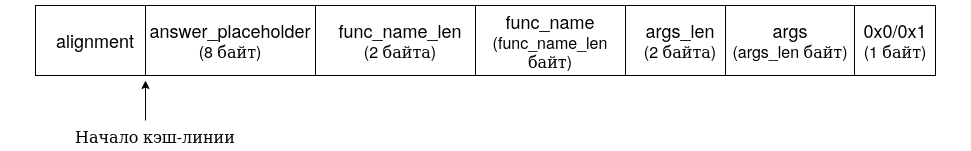
\includegraphics[width=\linewidth]{stack_frame.png}
\end{figure}

Маркер конца фрейма (\texttt{0x0}) или стека (\texttt{0x1}) позволяет нам понять, был ли прочитанный из персистентного стека фрейм последним или дальше на стеке расположен ещё хотя бы один стековый фрейм.

Таким образом, размер используемой части фрейма равен $8 + 2 + \texttt{func\_name\_len} + 2 + \texttt{args\_len} + 1 =$ $= 13 + \texttt{func\_name\_len} + \texttt{args\_len}$ байт. Пустые байты в начале фрейма не используются и нужны только для того, чтобы используемая части фрейма была выровнена по размеру кэш-линии.

\section{Обновление персистетного стека}

Персистентный стек нужно обновлять при вызове новой функции (в этом случае, нужно добавить на вершину стека новый стековый фрейм) и при выходе из функции (в таком случае нужно убрать один стековый фрейм с вершины стека).

Будем называть последним фреймом тот фрейм, который является последним на момент до начала записи нового стекового фрейма. Например, в примере ниже (см. Рисунок~\ref{stack-add-pic}), фрейм 3~--- это новый фрейм, а фрейм 2~--- последний фрейм.

Перед входом в функцию будем делать следующие действия (см. Рисунок \ref{before-function-call}):

\begin{figure}[H]
  \centering
  \caption{До вызова функции}
  \label{before-function-call}
  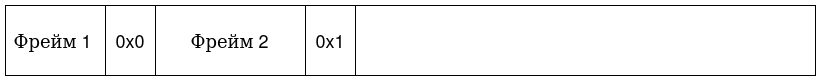
\includegraphics[width=\linewidth]{3.png}
\end{figure}

\begin{itemize}
    \item После маркера конца стека пишем новый стековый фрейм, завершая его маркером конца стека (см. Рисунок \ref{stack-add-pic}). Новый стековый фрейм располагается после маркера конца стека, которым завершается последний фрейм, поэтому он пока не считается стековым фреймом. 
    
    \begin{figure}[H]
      \centering
      \captionof{figure}{После добавления нового стекового фрейма после конца стека}
      \label{stack-add-pic}
      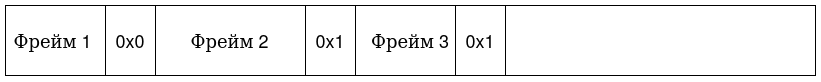
\includegraphics[width=\linewidth]{4.png}
    \end{figure}

    
    \item У последнего стекового фрейма меняем маркер конца стека на маркер конца фрейма (см. Рисунок \ref{after-moving-forward}). При этом последний фрейм становится предпоследним, а новый фрейм становится последним, тем самым происходит перемещение конца стека вперёд.
    
     \begin{figure}[H]
      \centering
      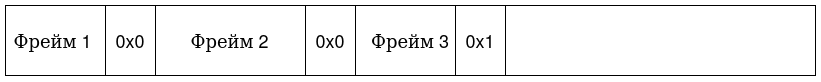
\includegraphics[width=\linewidth]{5.png}
      \captionof{figure}{После перемещения конца стека вперёд}
      \label{after-moving-forward}
    \end{figure}
\end{itemize}

\bigbreak
\bigbreak

Перед выходом из функции будем делать следующие действия (см. Рисунок \ref{before-return-pic}):

\begin{figure}[H]
  \centering
  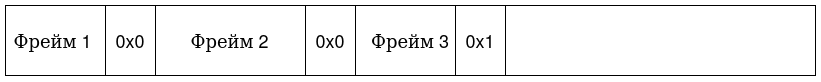
\includegraphics[width=\linewidth]{5.png}
  \captionof{figure}{До выхода из функции}
  \label{before-return-pic}
\end{figure}

\begin{itemize}
    \item У предпоследнего стекового фрейма меняем маркер конца фрейма на маркер конца стека (см. Рисунок \ref{after-moving-backward-pic}). При этом предпоследний стековый фрейм становится последним, а последний стековый фрейм становится набором произвольных данных, расположенных после конца стека, то есть происходит перемещение конца стека назад.
    
    \begin{figure}[H]
      \centering
      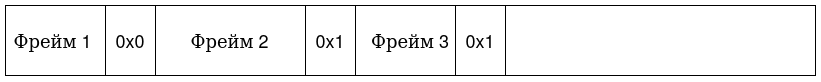
\includegraphics[width=\linewidth]{4.png}
      \captionof{figure}{После перемещения конца стека назад}
      \label{after-moving-backward-pic}
    \end{figure}
\end{itemize}

В вышеприведённом алгоритме при выходе из функции необходимо у предпоследнего стекового фрейма заменить маркер конца фрейма на маркер конца стека. Из этого следует, что если предпоследнего фрейма не существует (то есть фрейм, который мы собираемся убрать со стека, является единственным фреймом на стеке), убрать текущий фрейм со стека невозможно. Поэтому первый фрейм, хранимый на стеке, никогда не должен удаляться со стека. Есть два способа добиться этого:

\begin{itemize}
    \item Считать, что первый фрейм, хранимый на стеке, является фиктивным и не соответствует никакой функции. Этот фиктивный фрейм будет добавляться на стек до начала работы системы и никогда не будет удаляться с вершины стека.
    
    \item Потребовать, чтобы первая функция, которая будет запущена в каждом потоке, никогда не завершалась. Единственным способом прервать работу этой функции будет сбой системы. Так как первая вызванная в каждом потоке функция никогда не завершается, то и убирать первый стековый фрейм будет не нужно. В дальнейших главах будет рассмотрена архитектура системы и будет показано, что данное ограничение не является недостатком дизайна, а наоборот, отвечает всем накладываемым на систему требованиям.
\end{itemize}


\section{Атомарность входа и выхода}

Заметим, что стековый фрейм может не влезть в одну кэш-линию (например потому, что функция получает массив аргументов длиной больше, чем размер кэш-линии). Так как на системах с NVRAM запись в NVRAM нескольких кэш-линий неатомарна, то и запись такого фрейма на стек не будет атомарна.

Следовательно, в ходе записи нового стекового фрейма может произойти сбой, который позволит записать только часть нового стекового фрейма, но не позволит записать остаток фрейма. Например, если сбой произойдёт после записи первой кэш-линии, но до записи всех остальных, новый персистентный стековый фрейм будет записан не полностью.

Заметим, что в процессе записи мы сначала пишем на стек новый стековый фрейм, и только после того, как запись нового фрейма завершилась успешно, мы перемещаем конец стека вперёд (то есть заменяем у последнего стекового фрейма маркер конца стека на маркер конца фрейма). В таком случае, заметим, что вышеописанный  сбой может произойти только до перемещения конца стека вперёд, то есть до того, как мы поменяем у последнего фрейма маркер конца стека на маркер конца фрейма. Из этого следует, что не полностью записанный стековый фрейм будет располагаться за концом стека и вообще не будет интерпретироваться как стековый фрейм. То есть в случае такого сбоя мы считаем, что сбой произошёл до входа в функцию и функция вообще не была вызвана в этом потоке. (см. Рисунок~\ref{corrupted-frame-pic})

\begin{figure}[H]
  \centering
  \caption{Фрейм, при записи которого произошёл сбой, располагается за концом стека}
  \label{corrupted-frame-pic}
  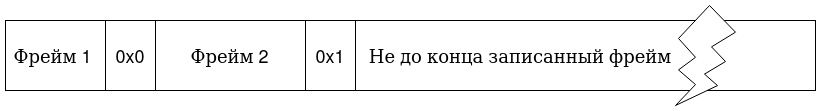
\includegraphics[width=\linewidth]{corrupted_frame.png}
\end{figure}

Заметим также, что перемещение конца стека вперёд сводится к записи в NVRAM одного байта (у последнего фрейма маркер конца стека заменяется на маркер конца фрейма). Точно так же перемещение конца стека назад аналогично сводится к записи в NVRAM одного байта (у предпоследнего фрейма маркер конца фрейма заменяется на маркер конца стека). А так как один байт всегда лежит строго в одной кэш-линии и никогда не пересекает её границ, перемещение конца стека сводится к сбросу в NVRAM единственной кэш-линии (в которой лежит изменённый байт), всегда выполняется атомарно, следовательно, в процессе перемещения конца стека сбой произойти не может.

Если же сбой происходит после перемещения конца стека вперёд/назад, но до реального исполнения процессором команды \texttt{CALL}/\texttt{RET}, считаем, что вход/выход в/из функции был успешно выполнен и команда \texttt{CALL}/\texttt{RET} была успешно исполнена. Действительно, исполнение команд \texttt{CALL} и \texttt{RET} не приводят к записи данных в NVRAM, поэтому после возобновления работы системы ситуация, при которой они были выполнены (и сбой произошёл сразу после выполнения одной из этих команд процессором), неотличима от ситуации, при которой они не были выполнены (то есть сбой произошёл сразу после перемещения конца стека, до исполнения процессором одной из этих команд). В таком случае, будем всегда считать, что вызов функции и возврат из неё происходят в момент перемещения конца стека.

Заметим, что для корректности поддержания стека мы требуем от железа даже не атомарности записи кэш-линии, а всего лишь атомарности записи одного байта (чтобы перемещение конца стека происходило атомарно). Это позволяет эмулировать процесс запуска алгоритмов для NVRAM на более дешёвом железе (например, на жёстких дисках). Современные жёсткие диски могут не гарантировать атомарности записи кэш-линии, зато гарантируют атомарность записи одного байта.

Чтобы вышеприведённые рассуждения были корректны, ни одна запись в персистентный стек не должна быть отложена из-за попадания в кэш. Поэтому сразу после записи любых данных на стек необходимо производить сброс кэш-линии, в которую попала записанные данные, в NVRAM. В противном случае возможна одна из следующих ситуаций:

\begin{itemize}
    \item При перемещении конца стека вперёд мы пишем маркер конца фрейма вместо маркера конца стека в последний фрейм. Представим, что этот маркер попал в кэш и не записался в NVRAM (см. Рисунок \ref{marker-not-flushed-pic}). Теперь мы вызываем функцию, соответствующую новому стековому фрейму, и эта функция пишет что-то в NVRAM, причём запись попадает туда сразу, минуя кэш (например, в коде функции записанные данные явно сбрасываются в NVRAM из кэша). Если в этот момент (то есть до того, как маркер конца фрейма будет сброшен в NVRAM) произойдёт сбой, то после возобновления работы системы новый стековый фрейм будет располагаться за маркером конца стека, и, следовательно, мы будем считать, что не вызвали соответствующую ему функцию. Следовательно, \texttt{recover}-версия этой функции не будет вызвана. Несмотря на это, функция успела внести какие-то изменения в NVRAM и, не вызвав её \texttt{recover}-версию, мы неправильно проведём восстановление системы после сбоя.
    
    
    \begin{figure}[H]
      \begin{center}
      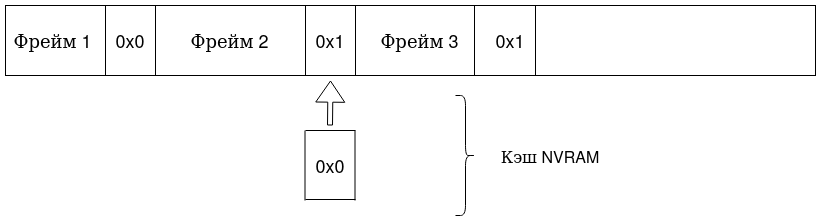
\includegraphics[width=\linewidth]{marker_not_flushed.png}
      \captionof{figure}{Функция, соответствующая фрейму 3, была вызвана и успела внести изменения в NVRAM, но 
      соответствующий ей фрейм расположен после конца стека,
      recover-функция не будет вызвана}
      \label{marker-not-flushed-pic}
      \end{center}
    \end{figure}
    
    \item Представим себе, что записанные в новый стековый фрейм аргументы вызываемой функции попали в кэш и не были сброшены в NVRAM. Теперь мы вызываем функцию, соответствующую новому стековому фрейму, и эта функция пишет что-то в NVRAM, причём запись попадает туда сразу, минуя кэш (например, в коде функции записанные данные явно сбрасываются в NVRAM из кэша). Если в этот момент (то есть до того, как аргументы вызванной функции будет сброшены в NVRAM) произойдёт сбой системы, после восстановления мы не будем знать, с какими аргументами была вызвана функция и, следовательно, не сможем вызвать \texttt{recover}-версию этой функции с теми же аргументами. Следовательно, мы не сможем корректно восстановить систему после сбоя.
\end{itemize}

\bigbreak

Заметим, что в начале каждого стекового фрейма расположены $0 \leq n < \texttt{CACHE\_LINE\_SIZE}$ неиспользуемых байт, записанное в которых значение нам не важно. Мы никогда не читаем и не интерпретируем эти байты, они нужны только для выравнивания поля для сохранения ответа по размеру кэш-линии. Тогда при сбросе нового стекового фрейма в NVRAM нужно сбрасывать в NVRAM не весь новый фрейм, а только  его используемую часть. В таком случае, сбрасывается в NVRAM всегда строго $13 + \texttt{func\_name\_len} + \texttt{args\_len}$ байт, выровненных по кэш-линии. В таком случае, если $13 + \texttt{func\_name\_len} + \texttt{args\_len} \leq \texttt{CACHE\_LINE\_SIZE}$, для сброса нового стекового фрейма в NVRAM понадобится всего одна операция сброса кэш-линии.

\section{Работа с указателями}

При работе с указателями на NVRAM мы сталкиваемся с проблемами, аналогичными тем, с которыми мы столкнулись при работе с указателями на функции.

Мы эмулируем NVRAM с помощью жёстких дисков. Эмуляция происходит следующим образом: сначала мы создаём файл нужного размера на жёстком диске, потом открываем его с помощью системного вызова \texttt{open(2)}, получая файловый дескриптор, соответствующий открытому файлу. Открыв файл, мы отображаем его в память с помощью системного вызова \texttt{mmap(2)}, тем самым получив возможность работать с байтоадресуемой памятью, запись в которую приводит к записи в постоянное хранилище \cite{mmap}.

Как и в случае с NVRAM, запись в память, выделенную с помощью \texttt{mmap} не всегда приводит к немедленной записи в постоянное хранилище. Записанные данные могут остаться в буфере  в ядре операционной системы, играющем для отображаемого в память файла ту же роль, что и кэш для NVRAM (то есть при сбое системы даные из буфера пропадают, не попадая в энергонезависимое хранилище). Так же, как и в случае со сбросом кэша в NVRAM, можно с помощью системного вызова \texttt{msync} явно потребовать сброса записанных данных из буфера в ядре операционной системы в энергонезависимое хранилище \cite{msync}. 

Будем хранить персистетный стек каждого процесса в собственном файле, и с помощью отдельного файла мы будем эмулировать кучу NVRAM. Таким образом, если в системе есть \texttt{N} потоков, мы будем использовать \texttt{N + 1} файл для эмуляции NVRAM: \texttt{N} для эмуляции стеков потоков и один для эмуляции кучи NVRAM.

Представим теперь ситуацию, при которой мы передали вызванной функции \texttt{f(void*)} указатель на участок в куче NVRAM в качестве аргумента. Так как аргументы вызываемой функции записываются на персистетный стек, то и передаваемый указатель на NVRAM также будет записан на стек. Пусть в момент работы функции \texttt{f(void*)} произошёл сбой системы, после чего работа системы была возобновлена, а процесс перезапущен. После перезапуска процесса мы вновь открываем файл, с помощью которого мы эмулируем кучу NVRAM, и отображаем его в память. Операционная система могла отобразить файл в другое место виртуальной памяти, отличное от того, куда он был отображён до сбоя. Это приведёт к тому, что лежащий на персистетном стеке адрес может более не указывать на кучу NVRAM. Следовательно, указатель, который мы передадим \texttt{f\_recover(void*)} не будет более указывать в кучу NVRAM, поэтому нам не удастся корректно восстановить систему восле сбоя.

Замена эмуляции NVRAM с помощью отображаемых в память файлов на настоящую NVRAM также может не решить эту проблему. Скорее всего, NVRAM будет представлять из себя отдельное устройство, отображаемое в произвольное место виртуальной памяти с помощью системного вызова \texttt{mmap(2)} или подобного ему (то есть вместо использования механизма отображения файла в память мы будем использовать механизм отображения устройства в память), что порождает те же проблемы, что и при эмуляции NVRAM с использованием жёстких дисков. 

Поэтому везде при работе с NVRAM будем хранить не абсолютные адреса объектов в NVRAM, а смещения от адреса начала отображения NVRAM в виртуальное адресное пространство. Адрес начала отображения NVRAM в виртуальное адресное пространство должен храниться в глобальной переменной \texttt{PMEM\_START\_ADDRESS} в энергозависимой памяти и инициализироваться каждый раз при старте системы. Например, при эмуляции NVRAM с использованием отображаемых в память файлов \texttt{PMEM\_START\_ADDRESS} будет инициализироваться результатом вызова \texttt{mmap}, а при работе с настоящей NVRAM~--- результатом вызова специальной функции, отображающей NVRAM в виртуальное адресное пространство.

Заметим, что смещения не зависят от конкретного значения \texttt{PMEM\_START\_ADDRESS}, поэтому их можно сохранять в энергонезависимой памяти и использовать как корректное смещение даже после перезапуска процесса.

В ходе исполнения программы смещения можно преобразовывать в абсолютные адреса (по которым мы и будем обращаться к NVRAM). Например, имея смещение от адреса начала отображения NVRAM в виртуальное адресное пространство, можно легко получить абсолютный адрес, прибавив смещение к \texttt{PMEM\_START\_ADDRESS}.

В обратную сторону, смещение же легко получается из абсолютного адреса с помощью вычитания из абсолютного адреса \texttt{PMEM\_START\_ADDRESS}.

\section{Возвращаемое значение}
\label{return-value}

Традиционно, на архитектуре \texttt{x86} возвращаемые из функций значения передаются вызывающей стороне либо в регистре общего назначения \texttt{EAX} (если возвращаемое значение является целым числом или указателем), либо в регистрах арифметического сопроцессора (если возвращаемое значение является числом с плавающей точкой). Например, именно таковы правила возврата значений в конвенции вызова \texttt{cdecl}, одной из самых распространённых конвенций вызова, используемых на архитектуре \texttt{x86} \cite{calling-conventions}.

Тем не менее, при работе с NVRAM возвращаемое значение функции нельзя возвращать в регистрах процессора, так как регистры процессора энергозависимы. Представим, что функция \texttt{Op} завершилась и записала возвращаемое значение в регистр \texttt{EAX}. После этого произошло перемещение конца стека назад (вследствие чего стековый фрейм, соответствующий функции \texttt{Op}, был выброшен с вершины стека), после чего была исполнена команда \texttt{RET}, и в этот момент произошёл сбой.

С одной стороны, сбой произошёл до того, как вызывающая сторона успела сохранить значение из энергозависимого регистра \texttt{EAX} в NVRAM, поэтому после возобновления работы системы возвращаемое значение будет потеряно. С другой стороны, сбой произошёл после перемещения конца стека назад, поэтому при анализе стека после возобновления работы системы операция \texttt{Op} будет считаться корректно завершившейся, и \texttt{Op.Recover} не будет вызвана. Вследствие этого, возвращаемое значение операции \texttt{Op} будет потеряно навсегда и восстановить его не будет возможности. Следовательно, мы не сможем корректно восстановить систему после сбоя.

Для борьбы с проблемой такого рода необходимо записывать возвращаемое значение в NVRAM до того, как произойдёт перемещение конца стека назад.

Делать это можно следующим образом:

\begin{itemize}
    \item Перед вызовом функции вызывающая сторона выделяет память в NVRAM, доступ к которой имеет только один процесс.
    
    \item Вызывающая сторона передаёт указатель на эту память вызываемой функции в качестве параметра.
    
    \item Перед завершением вызываемая функция сохраняет по этому адресу ответ и производит сброс ответа из кэша в NVRAM.
    
    \item Только после завершения сброса кэшей происходит перемещение конца стека назад.
\end{itemize}

\bigbreak

Важно иметь в виду, что перемещение конца стека назад происходит не просто после записи возвращаемого значения в NVRAM, а после сброса возвращаемого значения из кэша в NVRAM. В противном случае, мы столкнёмся с проблемой, аналогичной той, с которой мы столкнулись, возвращая значение в энергозависимых регистрах.

Представим, что функция \texttt{Op} завершилась и записала возвращаемое значение в NVRAM, но при этом не сбросила кэши и возвращаемое значение осталось в кэше, не попав в NVRAM. После этого произошло перемещение конца стека назад (вследствие чего стековый фрейм, соответствующий функции \texttt{Op}, был выброшен с вершины стека), после чего была исполнена команда \texttt{RET}, и в этот момент произошёл сбой.

С одной стороны, сбой произошёл до того, как возвращаемое значение попало из кэша в NVRAM, поэтому после возобновления работы системы возвращаемое значение будет потеряно. С другой стороны, сбой произошёл после перемещения конца стека назад, поэтому при анализе стека после возобновления работы системы операция \texttt{Op} будет считаться корректно завершившейся, и \texttt{Op.Recover} не будет вызвана. Вследствие этого, возвращаемое значение операции \texttt{Op} будет потеряно навсегда и восстановить его не будет возможности. Следовательно, мы не сможем корректно восстановить систему после сбоя.

\section{Возврат значения на стеке}
\label{return-value-stack}

Кроме описанного выше способа возврата значения, существуют и другие. Например, значение можно возвращать на стеке.

Будем в начале каждого стекового фрейма, в качестве первого поля фрейма, сохранять восемь байт под ответ. Если функция \texttt{G}, вызванная из функции \texttt{F} хочет записать ответ на стек NVRAM, она должна записать ответ в начало предыдущего стекового фрейма~-- это будет стековый фрейм, соответствующий функции \texttt{F} (см. Рисунок~\ref{write-answer-pic}) ~-- и сбросить возвращаемое значение из кэша в NVRAM (в предыдущей главе было описано, почему функция должна сбрасывать собственное возвращаемое значение из кэша в NVRAM до того, как произойдёт перемещение конца стека назад). 

\begin{figure}[H]
  \centering
  \caption{Запись возвращаемого значения в начало предыдущего фрейма}
  \label{write-answer-pic}
  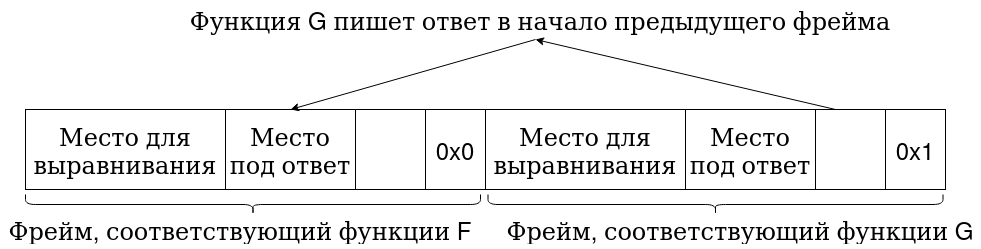
\includegraphics[width=\linewidth]{write_answer.png}
\end{figure}

Функция \texttt{F} может получить ответ функции \texttt{G} после её завершения, для этого достаточно прочитать первые восемь байт собственного стекового фрейма.

Разумеется, если функция \texttt{F} после завершения работы функции \texttt{G} вызовет возвращающую ответ функцию \texttt{H}, то после завершения работы функции \texttt{H} в начале стекового фрейма, соответствующего функции \texttt{F}, будет записан ответ функции \texttt{H}, а ответ функции \texttt{G} будет стёрт. Если функции \texttt{F} необходимо сохранить возвращаемое значение функции \texttt{G}, она должна сделать это явно, перед вызовом функции \texttt{H} перенеся возвращаемое значение из начала собственного стекового фрейма в заранее выделенный в куче NVRAM участок памяти.

Так как мы хотим, чтобы запись возвращаемого значения выполнялась атомарно, мы выполним выравнивание адреса начала возвращаемого значения в каждом стековом фрейме по размеру кэш-линии. Именно для этого в начале каждого фрейма мы пропускаем $0 \leq n <  \texttt{CACHE\_LINE\_SIZE}$ неиспользуемых байт. Так как адрес начала возвращаемого значение выровнен по размеру кэш-линии (см. Рисунок \ref{answer-aligmnent-pic}), запись возвращаемого значения сводится к записи восьми байт, лежащих строго в одной кэш-линии и не пересекающих её границ (разумеется, для этого размер кэш-линии должен быть не меньше восьми байт ~--- к счастью, на архитектуре \texttt{x86} размер кэш-линии равен 64 байтам), поэтому в системах с NVRAM такая операция выполняется атомарно.

\begin{figure}[H]
  \centering
  \caption{Положение места для записи возвращаемого значения в кэш-линии архитектуры x86}
  \label{answer-aligmnent-pic}
  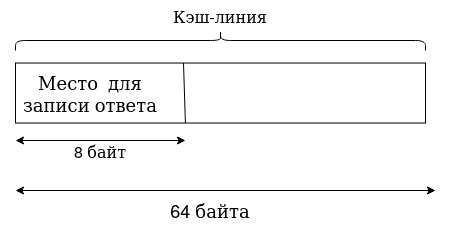
\includegraphics[width=\linewidth]{answer_in_cacheline.png}
\end{figure}

В вышеприведённом алгоритме функция пишет возвращаемое значение в начало предыдущего стекового фрейма. Из этого следует, что если предыдущего фрейма не существует (то есть фрейм, соответствующий исполняемой в данный момент функции, является единственным фреймом на стеке), вернуть значение из исполняющейся в данный момент функции невозможно. Как и в случае с запретом на удаление первого фрейма со стека, есть два способа добиться того, чтобы  функция, соответствующая первому фрейму, никогда не возвращала ответ:

\begin{itemize}
    \item Считать, что первый фрейм, хранимый на стеке, является фиктивным и не соответствует никакой функции. Так как первый фрейм не соответствует никакой функции, то и вернуть значение функция, соответствующая ему, не может.
    
    \item Потребовать, чтобы первая функция, которая будет запущена в каждом потоке, никогда не завершалась. Единственным способом прервать работу этой функции будет сбой системы. Так как первая вызванная в каждом потоке функция никогда не завершается, то и возвращать из неё значение не нужно. В дальнейших главах будет рассмотрена архитектура системы и будет показано, что данное ограничение не является недостатком дизайна, а наоборот, отвечает всем накладываемым на систему требованиям.
\end{itemize}

К сожалению, жёсткие диски не предоставляют гарантию атомарности записи кэш-линии, поэтому на системах, использующих жёсткие диски в качестве энергонезависимого хранилища, может произойти сбой в процессе записи ответа, в результате которого ответ будет записан не целиком. Пользовательский код самостоятельно должен учитывать возможность такого сбоя. Например, для борьбы с такими сбоями можно использовать следующий протокол:

\begin{itemize}
    \item Перед записью нового фрейма на стек запишем в каждый из восьми байт места под ответ текущего стекового фрейма значение по умолчанию (например, \texttt{0xFF}). Подразумевается, что ни один байт ответа не может быть равен этому значению.
    
    \item Вызываемая функция пишет ответ на стек обычным образом.
    
    \item \texttt{recover}-версия вызываемой функции первым делом читает ответ с предыдущего фрейма.
    
    \item Дальше возможны три варианта:
        \begin{itemize}
            \item Все байты ответа содержат значение по умолчанию. Следовательно, сбой произошёл до того, как ответ был записан на персистентный стек, необходимо провести восстановление.
            
            \item Ни один из байт ответа не содержит значения по умолчанию. Следовательно, сбой произошёл уже после того, как ответ был записан на персистентный стек. Восстановления производить не нужно, \texttt{recover}-функция тут же может завершить свою работу.
            
            \item Только часть байт ответа содержит значения по умолчанию. Следовательно, сбой произошёл в процессе записи ответа на персистентный стек, необходимо провести восстановление.
        \end{itemize}
\end{itemize}

Заметим, что если ответ функции занимает один байт (например, ответ функции \texttt{CAS} занимает всего один байт) и ответ пишется в первый байт персистентного фрейма, то сбой в процессе записи ответа невозможен даже при эмуляции алгоритма на жёстких дисках (так как жёсткие диски предоставляют гарантию атомарности записи одного байта).

\section{Взаимодействие с пользователем}

Для работы с системой запуска программ для NVRAM от пользователя требуется выполнять следующие действия:

\begin{itemize}
    \item Для всех функций, имеющих доступ к NVRAM, предоставлять \texttt{recover}-версию. Эта версия должна принимать те же аргументы, что и обычная функция
    
    \item Все такие функции должны принимать аргументы, сериализованные в массив байт и иметь сигнатуру
        
        \texttt{void func(const uint8\_t* args)}
        
        
        \texttt{void func\_recover(const uint8\_t* args)} 
        
    При вызове функции пользователь сам должен сериализовать передаваемые ей аргументы в массив байт, а также десериализовывать аргументы, получаемые пользовательской функцией, из массива байт.

    \item Вызывать функции, работающие с NVRAM, нельзя напрямую. Нужно делать это через функцию \texttt{void do\_call(std::string const& func\_name, std::vector<uint8\_t> const& args)}. Эта функция до вызова пользовательской функции создаёт стековый фрейм и производит перемещение конца стека вперёд, а после завершения пользовательской функции производит перемещение конца стека назад.
    
    \item Перед завершением функции нужно самостоятельно сохранять ответ в NVRAM. Сохранение ответа на стек производится с помощью функции \texttt{void write\_answer(std::vector<uint8\_t> const& answer)}, сохранение в кучу NVRAM пользователь должен делать самостоятельно, используя описанный в секции \ref{return-value} протокол. Для чтения ответа с текущего стекового фрейма (то есть ответа, записанного функцией, только что завершившей свою работу) можно использовать функцию \texttt{std::vector<uint8\_t> read\_answer(uint8\_t size)}, а для чтения ответа с предыдущего стекового фрейма (то есть ответа, записанного функцией, исполняющейся в данный момент) можно использовать функцию \texttt{std::vector<uint8\_t> read\_current\_answer(uint8\_t size)}.
    
    \item Перед началом работы регистрировать в глобальной хеш-таблице все используемые функции, запоминая по имени функции адрес самой функции и адрес её \texttt{recover}-версии. В дальнейшем можно использовать только заранее зарегистрированные функции.
    
    \item Самостоятельно передавать указатели на кучу NVRAM как смещения от адреса начала отображения NVRAM в виртуальное адресное пространство. При необходимости получить данные по указателю необходимо самостоятельно прибавлять смещение к \texttt{PMEM\_START\_ADDRESS}, получая абсолютный адрес; при необходимости получить смещение из абсолютного адреса~--- вычитать из абсолютного адреса \texttt{PMEM\_START\_ADDRESS}. Пользователь должен самостоятельно заботиться о том, чтобы нигде в NVRAM не сохранялись указатели на кучу NVRAM вместо смещений.
\end{itemize}

\section{Архитектура системы}

Система состоит из главного потока и \texttt{N} рабочих потоков.

Главный поток может быть запущен в двух режимах: в штатном режиме и в режиме восстановления.

При запуске в штатном режиме главный поток:

\begin{itemize}
    \item Инициализирует кучу NVRAM: создаёт на жёстком диске файл требуемого размера, с помощью которого будет производиться эмуляция кучи, открывает его и отображает в память, сохраняет в переменной \texttt{PMEM\_START\_ADDRESS} адрес начала отображения файла в виртуальное адресное пространство.
    
    \item Если это первый запуск, главный поток инициализирует аллокатор памяти (вопрос выделения памяти в куче NVRAM будет рассмотрен в главе \ref{nvram-allocation}).
    
    \item Регистрирует в глобальной хеш-таблице имена и адреса всех функций (и их \texttt{recover}-версий), которые будут использоваться в ходе исполнения.
    
    \item Создаёт \texttt{N} персистетных стеков. При эмуляции NVRAM с помощью жёстких дисков аллоцировать можно как каждый стек в собственном файле, так и все стеки в единственном файле (в таком случае каждый рабочий поток получит указатель на различные смещения в одном и том же файле). При реализации системы я решил аллоцировать каждый стек в собственном файле, чтобы ошибки при реализации алгоритма работы с персистентным стеком одного рабочего потока не приводили к повреждению персистентных стеков других рабочих потоков.
    
    \item Запускает \texttt{N} рабочих потоков и выдаёт каждому рабочему потоку указатель на начало его персистетного стека.
    
    \item Добавляет задачи, которые будут исполнять рабочие потоки, в очередь задач. В качестве очереди задач использовалась обычная очередь из стандартной библиотеки языка \texttt{C++}, защищённая грубой блокировкой для корректной работы в многопоточном окружении. Также при реализации очереди использовались мониторы Хоара \cite{hoare-monitor} для того, чтобы рабочий поток мог пассивно ожидать появления задач в очереди при попытке взять задачу из пустой очереди, а главный поток мог оповестить рабочий поток о том, что в очереди появилась новая задача при добавлении задачи в очередь. Очередь не является персистентной и располагается в энергозависимой памяти.
\end{itemize}

\bigbreak

Запуску в режиме восстановления предшествует сбой системы. При запуске в режиме восстановления главный поток:

\begin{itemize}
    \item Инициализирует кучу NVRAM: открывает файл и отображает его в память, сохраняет в переменной \texttt{PMEM\_START\_ADDRESS} адрес начала отображения файла в виртуальное адресное пространство. Аллокатор при этом не инициализируется, так как он был инициализирован при запуске в штатном режиме.
    
    \item Регистрирует в глобальной хеш-таблице имена и адреса всех функций (и их \texttt{recover}-версий), которые будут использоваться в ходе исполнения.
    
    \item Открывает файлы, соответствующие персистентным стекам рабочих потоков, исполнявшихся во время сбоя и отображает их в память.
    
    \item Запускает \texttt{N} восстанавливающих потоков и выдаёт каждому из восстанавливающих потоков указатель на соответствующий персистетный стек, открытый на предыдущем шаге. Так как каждому восстанавливающему потоку выдаётся ровно один стек рабочего потока, число восстанавливающих потоков в системе должно быть равно числу рабочих потоков.
    
    \item Дожидается завершения всех восстанавливающих потоков и после этого перезапускается в штатном режиме. Заметим, что этот запуск в штатном режиме не будет являться первым запуском в штатном режиме. В частности, аллокатор памяти уже будет инициализирован и не нужно будет инициализировать его повторно.
\end{itemize}

\bigbreak

Рабочие потоки при этом разделяют очередь задач и исполняют эти задачи.

Задача содержит описание того, что необходимо сделать (например, там может быть указано, что необходимо выполнить операцию \texttt{CAS} по переменной, лежащей в куче NVRAM по смещению \texttt{0x2517} с аргументами \texttt{expected = 100, new = 200}) и указатель на выделенную в NVRAM память, куда пишется результат исполнения описанной операции. Эта память инициализируется главным потоком при создании задачи и доступна всего двум потокам: рабочий поток, исполняющий задачу, единственный раз пишет в неё результат исполнения операции, а главный поток читает эту память для того, чтобы узнать результат.

Изначально эта память инициализируется значением по умолчанию, которое не может быть результатом исполнения задачи (например, для \texttt{CAS} значением по умолчанию может стать \texttt{-1}, а возможными результатами исполнения~--- \texttt{0} и \texttt{1}). Сравнивая текущее записанное в переменной значение со значением по умолчанию, главный поток может узнать, закончилось ли выполнение задачи. Если исполнение задачи закончилось, главный поток более не будет обращаться к этой памяти. В противном случае, главный поток обратится к этой памяти ещё раз через какое-то время чтобы ещё раз узнать, завершилось ли исполнение задачи.

Вспомним, что первый фрейм, расположенный на персистетном стеке, не может быть удалён со стека. Следовательно, функция, котрая была вызвана первой в каждом из рабочих потоков, никогда не должна завершаться. Кроме того, вспомним, что ответ функции всегда пишется на предыдущий стековый фрейм, следовательно, первая вызванная в каждом потоке функция не должна возвращать ответ.

Заметим, что эти ограничения удовлетворяют архитектуре системы. Функция, которая вызывается первой в каждом из рабочих потоков, в бесконечном цикле ожидает, используя очередь, заданий от главного потока и исполняет эти задания. Эта функция никогда не завершается нормальным образом, никогда не возвращает ответ, единственным способом завершить работу этой функции является сбой системы.

Заметим, что эта функция никак не взаимодействует с NVRAM. Тем не менее, мы будем создавать для неё стековый фрейм на персистентном стеке (это будет первый фрейм на стеке каждого потока), который мы никогда не будем удалять с персистентного стека. Так как функция никак не взаимодействиует с NVRAM, её \texttt{recover}-версия не производит никаких действий и тут же завершается.

\section{Восстановление после сбоя}

При сбое системы мы для начала устраняем проблемы оборудования, если нужно (например, включаем питание), после чего перезапускаем систему.

Мы запускаем \texttt{N} восстанавливающих потоков~--- по одному восстанавливающему потоку на каждый рабочий поток. Каждому восстанавливающему потоку мы предоставляем ссылку на персистентный стек соответствующего рабочего потока.

После чего каждый восстанавливающий поток проходится по собственному стеку от конца к началу, исполняя \texttt{recover}-операцию для каждого персистентного стекового фрейма. По завершении \texttt{recover}-операции поток перемещает конец стека назад и повторяет эти действия до тех пор, пока его стек не опустеет.

Таким образом, восстановление происходит параллельно, что позволяет осуществлять потенциально более быстрое восстановление, чем восстановление в один поток.

Если в процессе восстановления произойдёт повторный сбой, то после возобновления работы системы восстановление после повторного сбоя начнётся с того места, где прервалось восстановление в прошлый раз (см. Рисунок \ref{repeatable-crash-pic}). Заметим, что при завершении каждой \texttt{recover}-операции восстанавливающий поток передвигает конец стека назад, тем самым уменьшая размер стека с каждой выполненной \texttt{recover}-операцией. Таким образом, при восстановлении в системе всегда есть прогресс, даже при повторных сбоях.

\begin{figure}[H]
  \centering
  \caption{Восстановление системы в условиях повторных сбоев}
  \label{repeatable-crash-pic}
  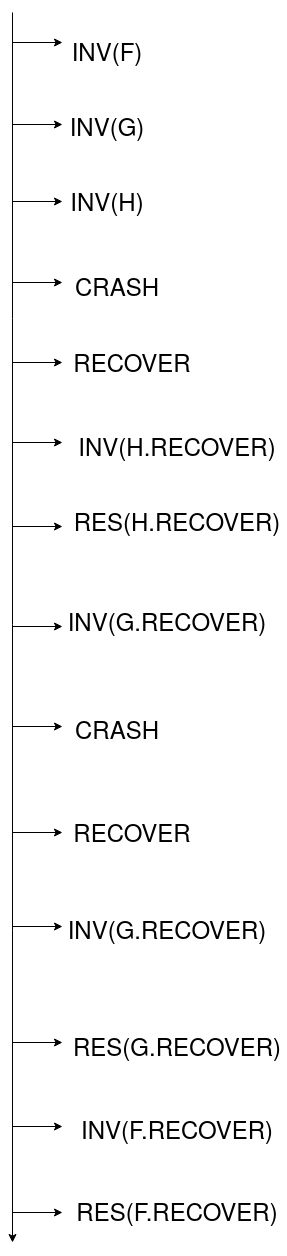
\includegraphics[scale=0.5]{repeatable_crash.png}
\end{figure}


\section{Использование алгоритма для запуска программ, удовлетворяющих более слабым условиям корректности}

Заметим, что при запуске кода, удовлетворяющего условию корректности \emph{nesting-safe recoverable linearizability} нет разницы между завершением операции \texttt{Op} и завершением операции \texttt{Op.Recover}. Если некая операция была завершена, то для вызывающего эту операцию кода не должно быть разницы, завершилась она со сбоем или нет.

Однако, существуют условия корректности, в которых эта разница значительна. Рассмотрим, например, условие корректности \emph{durable linearizability}, описанное в секции \ref{crush-models}. Это условие корректности требует, чтобы после восстановления системы после сбоя был виден эффект всех операций, исполнение которых завершилось до сбоя. Если же операция исполнялась в момент сбоя, то результат её работы может быть как виден, так и не виден.

Существует очевидный способ написать код, удовлетворяющий этому условию корректности: пусть каждой операции \texttt{Op}, в коде которой происходит доступ к NVRAM, будет сопоставлена операция \texttt{Op.Cleanup}, которая получает те же аргументы, что и исходная операция. В случае сбоя системы \texttt{Op.Cleanup} должна откатить обратно все изменения, которые были внесены в NVRAM в ходе исполнения операции \texttt{Op}. Тогда \texttt{cleanup}-версии всех операций, исполнявшихся в момент сбя, откатят изменения, которые внесли в NVRAM эти операции до сбоя, и после восстановления системы эффект этих операций будет не виден.

В таком случае, очевидно, исполняя \texttt{Op.Cleanup} по тем же правилам, по которым мы исполняли \texttt{Op.Recover}, мы получим возможность запускать код, удовлетворяющий условию корректности durable linearizability, для этого нам даже не нужно будет менять ни строчки в коде алгоритма запуска и восстановления.

Кроме того, в коде, удовлетворяющем условию корректности \emph{durable linearizability}, после восстановления системы должен быть виден эффект всех операций, исполнение которых завершилось до момента сбоя. Для этого каждая операция \texttt{Op} перед завершением должна сбросить в NVRAM все кэш-линии, которые были изменены в ходе исполнения этой операции.

Условие корректности \emph{buffered durable linearizability} отличается от \emph{durable linearizability} только тем, что после восстановления системы эффект части операций, завершившихся до сбоя, может быть не виден. Но в таком случае объект, операции с которым удовлетворяют условию корректности \emph{buffered durable linearizability}, должен предоставлять операцию \texttt{sync()}. Если исполнение этой операции завершилось до сбоя, то после восстановления системы должны быть видимы эффекты всех операций, исполнение которых завершилось до вызова \texttt{sync()}. Эффекты исполнения операций, исполнение которых завершилось после вызова \texttt{sync()}, но до сбоя, а также тех операций, которые исполнялись в момент сбоя, могут быть не видимы после восстановления системы.

Алгоритм запуска программ, удовлетворяющих этому условию корректности, не отличается от алгоритма запуска программ, удовлетворяющих условию \emph{durable linearizability}. Но, в отличие от \emph{durable linearizability}, операции, удовлетворяющие условию \emph{buffered durable linearizability} не обязаны перед завершением работы производить сброс в NVRAM всех кэш-линий, изменённых в процессе операции. Операция \texttt{sync()} должна быть реализована таким образом, что все кэш-линии, изменённые до момента вызова операции \texttt{sync()}, перед завершением этой операции должны быть сброшены в NVRAM из кэша.

\section{Реализация алгоритма}

Заметим, что разработанный алгоритм требует от энергонезависимого хранилища гарантию атомарности записи всего одного байта. Жёсткие диски, в отличие от NVRAM, могут не предоставлять гарантию атомарной записи целой кэш-линии, но они гарантируют атомарность записи одного байта. Именно поэтому разработанный алгоритм можно реализовывать не только на системе с использованием NVRAM, но и на системе, использующей жёсткие диски в качестве энергонезависимого хранилища. 

При реализации алгоритма в качестве базовового примитива многопоточного исполнения будем использовать потоки, а не процессы, по следующим причинам:

\begin{itemize}
    \item Все потоки одного процесса разделяют память, вследствие чего при использовании потоков можно, например, с лёгкостью использовать разделяемую очередь заданий, расположенную в общей для всех потоков памяти. Разделение же памяти между процессами потребовало бы использования продвинутых механизмов межпроцессного взаимодействия, в частности shared memory-mapped files \cite{mmap}, pipes \cite{pipe}, POSIX message queues \cite{posix-mq}, file locking \cite{file-locking}, POSIX named semaphores \cite{posix-sems}.
    
    \item Все потоки одного процесса могут быть с лёгкостью немедленно остановлены с помощью посылания сигнала \texttt{SIGKILL} этому процессу. Так как сигнал \texttt{SIGKILL}, посланный процессу, не может быть перехвачен и обработан и этот сигнал немедленно завершает процесс, именно с помощью посылания процессу этого сигнала можно эмулировать сбои системы. В противоположность использованию потоков, несколько процессов не могут быть легко остановлены с использованием всего олного сигнала.
\end{itemize}

\bigbreak

Алгоритм был реализован на языке программирования \texttt{C++}. Этот язык обладает очень высокой производительностью и богатыми выразительными возможностями, позволяющими реализовывать (и, что тоже очень важно, правильно типизировать) высокоуровневые абстракции, такие как \texttt{shared\_ptr}, \texttt{weak\_ptr} и \texttt{unique\_ptr} (освобождающие программиста от необходимости управлять памятью вручную) или \texttt{variant} (позволяющий программисту использовать алгебраические типы). Кроме того, этот язык обладает богатым набором библиотек для решения различных посведневных задач (например, при реализации системы для написания тестов использовалась библиотека \texttt{gtest} \cite{gtest}). Кроме того, этот язык позволяет напрямую использовать системные вызовы операционной системы Linux.

При реализации алгоритма использовалась библиотека \texttt{PMDK}, облагчающая работу с энергонезависимой памятью \cite{pmdk}.

\chapterconclusion

В этой главе был разработан алгоритм запуска программ в NVRAM и восстановления системы после сбоя. В ходе проектирования алгоритма был разработан алгоритм обновления персистентного стека, рассмотрены вопросы атомарности входа в функцию и выхода из неё. Алгоритм был разработан с учётом возможности реализации на системе, использующей жёсткие диски в качестве энергонезависимого хранилища.

Была разработана архитектура системы, рассмотрена возможность повторных сбоев в ходе восстановления. Алгоритм разработан с учётом возможности повторных сбоев таким образом, чтобы алгоритм совершал прогресс даже при наличии в системе повторных сбоев.

Кроме того, были рассмотрены вопросы возврата значения из функций и корректной работы с адресами функций и указателями на NVRAM.

Рассмотренный апгоритм может быть использован для запуска программ, удовлетворяющих как условию корректности Nesting-safe recoverable linearizability, так и более слабым критериям корректности.

\chapter{Выделение памяти в куче NVRAM}
\label{nvram-allocation}

\section{Задача выделения памяти в куче NVRAM}

Задача выделения памяти в куче NVRAM состоит из:

\begin{itemize}
    \item Выделения динамической памяти произвольного размера в куче NVRAM с помощью функции \texttt{void* pmem\_alloc(size\_t size)}, принимающей в качестве параметра длину блока, который необходимо выделить в куче NVRAM (в байтах) и возвращающей указатель на первый байт этого блока.
    
    \item Освобождения динамической памяти в куче NVRAM с помощью функции \texttt{void pmem\_free(void* ptr)}, принимающей в качестве параметра указатель на первый байт блока, выделенного в куче NVRAM с помощью функции \texttt{pmem\_alloc}. Освобождаемый блок должен быть выделен в куче NVRAM с помощью функции \texttt{pmem\_alloc}, и на момент вызова функции \texttt{pmem\_free} этот блок не должен быть освобождён. Несоблюдение одного из этих условий приводит к неопределённому поведению.
\end{itemize}

\bigbreak

Таким образом, задача выделения памяти в куче NVRAM очень похожа на задачу выделения динамической памяти в куче RAM, решаемую, например, аллокатором \texttt{malloc} \cite{malloc}.

Подробнее задача выделения памяти в куче NVRAM рассматривается в статье \cite{cai2020understanding}.

Заметим, что в описанном в главе \ref{system-impl} алгоритме динамическую память нужно выделять только под ответ каждой задачи, исполняемой рабочими потоками. Если задача имеет ответ фиксированного размера, то можно написать более простой алгоритм, который к тому же не требует от системы гарантии атомарности записи кэш-линии (а только атомарности записи одного байта).

В этой главе рассмотрены два алгоритма выделения динамической памяти в куче NVRAM: первый алгоритм будет способен выделять память произвольного размера, но будет неспособен освобождать память, а также будет требовать от системы гарантии атомарности записи восьми байт. Второй алгоритм будет способен выделять блоки памяти только фиксированного размера, зато будет способен освобождать выделенную память и будет требовать от системы гарантии атомарности записи всего одного байта.

\section{Первый алгоритм}

Будем считать, что в каждый момент времени в куче NVRAM выделен непрерывный отрезок памяти со смещениями в диапазоне $[0; \texttt{CUR\_MAX\_OFFSET}]$. Следовательно, \texttt{CUR\_MAX\_OFFSET} определяет смещение последнего выделенного байта. Как и в предыдущеё главе, смещения будем считать от начала отображения кучи NVRAM (или файла, эмулирующего кучу NVRAM) в виртуальное адресное пространство.

Будем хранить \texttt{CUR\_MAX\_OFFSET} в начальных восьми байтах кучи NVRAM, то есть в отрезке памяти, имеющем смещения $[0; 7]$ (см. Рисунок~\ref{heap-structure-algorithm-1}). Следовательно, изначально \texttt{CUR\_MAX\_OFFSET} = 7. То есть при инициализации аллокатора необходимо в первые восемь байт кучи NVRAM записать число \texttt{7}.

\begin{figure}[H]
  \centering
  \caption{Структура кучи NVRAM в первом алгоритме аллокации}
  \label{heap-structure-algorithm-1}
  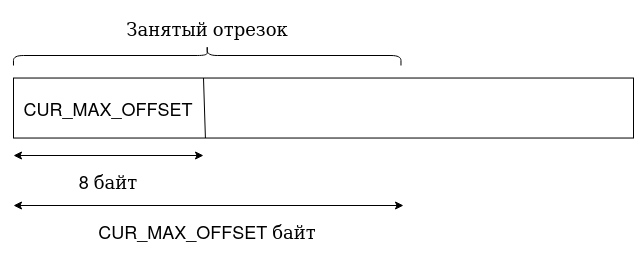
\includegraphics[scale=0.65]{allocation_first.png}
\end{figure}

При необходимости выделить блок памяти размером \texttt{size} байт:

\begin{itemize}
    \item Сохраним в локальную переменную \texttt{offset} текущее значение \texttt{CUR\_MAX\_OFFSET}, прочитав первые \texttt{8} байт кучи NVRAM. После этого шага в локальной переменной \texttt{offset} хранится смещение последнего выделенного в куче NVRAM байта.
    
    \item Так как текущий последний выделенный байт имеет смещение \texttt{offset}, после выделения блока памяти размером \texttt{size} байт последний выделенный байт будет иметь смещение \texttt{offset + size}. Следовательно, для выделения памяти запишем в первые \texttt{8} байт кучи NVRAM значение \texttt{offset + size}.
    
    \item Так как в переменной \texttt{offset} хранится смещение последнего выделенного байта, только что выделенный блок памяти будет начинаться со смещения \texttt{offset + 1}, именно это число и возвращает функция \texttt{pmem\_alloc}.
    
    \item Для того, чтобы предотвратить одновременный доступ нескольких потоков к аллокатору, будем защищать функцию \texttt{pmem\_alloc} грубой блокировкой, расположенной в энергозависимой памяти.
\end{itemize}

\bigbreak

Освобождение памяти не производится.

Рассмотрим псевдокод этого алгоритма (см. Листинг \ref{pmem-alloc-listing}).

\begin{algorithm}[H]
\caption{Псевдокод алгоритма выделения памяти}
\label{pmem-alloc-listing}
\begin{algorithmic}
    \Function{pmem\_alloc}{$size$}
        \State AllocatorLock.lock()
        \State uint64\_t cur\_max\_offset
        \State pmem\_read(0, \&cur\_max\_offset, 8)
        \State next\_max\_offset = cur\_max\_offset + size
        \State pmem\_write(0, \&next\_max\_offset, 8)
        \State pmem\_flush(0, 8)
        \State AllocatorLock.unlock()
        \State \Return cur\_max\_offset + 1
    \EndFunction
    
    \bigbreak
    \bigbreak

    
    \Function{pmem\_free}{$ptr$}
        \State \Return
    \EndFunction
\end{algorithmic}
\end{algorithm}

Заметим, что первые восемь байт кучи NVRAM выровнены по размеру кэш-линии (так как начало отображения файла или устройства в виртуальное адресное пространство выровнено по размеру страницы операционной системы \cite{mmap} и, следовательно, выровнено по размеру кэш-линии), следовательно, на NVRAM все первые восемь байт можно записать атомарно. Но для эмуляции NVRAM с помощью жёстких дисков имеет смысл разработать алгоритм, который бы работал корректно при наличии возможности атомарно записать только один байт.

\section{Второй алгоритм: инварианты, состояние аллокатора и структура кучи NVRAM}

Будем требовать от алгоритма выделять только блоки одного и того же размера (по $k$ байт каждый блок).

Разделим все байты на группы по $k + 1$ последовательных байт в каждой группе. Первые $k$ байт группы могут быть выделены пользователю, а последний байт группы хранит одно из трёх возможных состояний: \texttt{0x0}, \texttt{0x1} и \texttt{0x2} (см. Рисунок \ref{heap-structure-second-algo-pic}).

\begin{itemize}
    \item \texttt{0x0} в $(k + 1)$-ом байте блока означает, что этот блок выделен и пока не освобождён. Кроме того, дальше в куче NVRAM также есть выделенные, но не освобождённые блоки.
    
    \item \texttt{0x1} в $(k + 1)$-ом байте блока означает, что этот блок выделен и пока не освобождён. Кроме того, дальше в куче NVRAM все блоки свободны. Если $(k + 1)$-ый байт $N$-ого блока равен \texttt{0x1}, то дальнейшие блоки ($(N + 1)$-ый, $(N + 2)$-ой и так далее) свободны независимо от того, что написано в их $(k + 1)$-ых байтах.
    
    \item \texttt{0x2} в $(k + 1)$-ом байте блока означает, что этот блок освобождён и может быть выдан пользователю повторно. Кроме того, дальше в куче NVRAM также есть выделенные, но не освобождённые блоки.
\end{itemize}

\bigbreak

\begin{figure}[H]
  \centering
  \caption{Структура кучи NVRAM во втором алгоритме аллокации}
  \label{heap-structure-second-algo-pic}
  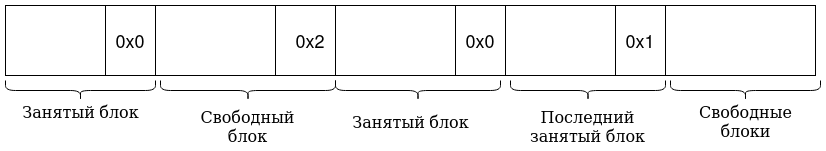
\includegraphics[width=\linewidth]{block_structure.png}
\end{figure}

В дальнейшем будем считать, что первый блок всегда занят (но указатель на него не выдаётся никому) и никогда не освобождается. Значит, в $(k + 1)$-ом байте кучи NVRAM всегда находится либо \texttt{0x0}, либо \texttt{0x1}. Таким образом, инициализация аллокатора состоит в необходимости записать \texttt{0x1} в $(k + 1)$-ый байт кучи NVRAM.

Состояние аллокатора характеризуется порядковым номером последнего выделенного блока (то есть такого блока, в $(k + 1)$-ом байте которого записано \texttt{0x1}) и множеством свободных блоков, расположенных слева от адреса начала последнего выделенного блока (то есть таких блоков, расположенных до начала последнего выделенного блока, в $(k + 1)$-ом байте которых записано \texttt{0x2}). И порядковый номер последнего выделенного блока (назовём это число границей аллокации) и множество свободных блоков расположены в энергозависимой памяти.

Как и в предыдущем случае, будем защищать аллокатор от двух и более одновременных запросов на выделение или освобождение памяти с помощью грубой блокировки, расположенной в энергозависимой памяти.

\section{Второй алгоритм: выделение памяти}

Если аллокатору приходит запрос на выделение блока памяти, возможны две ситуации:

\begin{itemize}
    \item Множество свободных блоков (то есть блоков, в $(k + 1)$-ом байте которых записано \texttt{0x2}) не пустое. В таком случае, необходимо взять произвольный блок из множества свободных блоков, в $(k + 1)$-ый байт этого блока записать \texttt{0x0} вместо \texttt{0x2}, удалить этот блок из множества свободных блоков и вернуть адрес его начала вызывающему.
    
    \item Множество свободных блоков пустое (см. Рисунок \ref{before-allocation-pic}). В таком случае необходимо сдвинуть границу аллокации вправо. Пусть текущая граница аллокации равна $N$. Для того, чтобы сдвинуть границу аллокации вправо, сначала запишем в $(k + 1)$-ый байт $(N + 1)$-ого блока \texttt{0x1} (см. Рисунок \ref{allocation-in-progress-pic}), а потом сменим значение $(k + 1)$-ого байта $N$-ого блока с \texttt{0x1} на \texttt{0x0} (см. Рисунок \ref{allocation-finished-pic}).
    
    \begin{figure}[H]
      \centering
      \caption{Структура кучи NVRAM до начала перемещения границы аллокации вправо}
      \label{before-allocation-pic}
      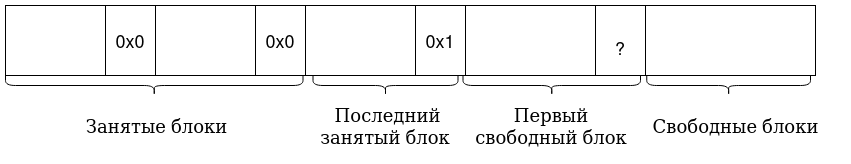
\includegraphics[width=\linewidth]{before_allocation.png}
    \end{figure}
    
    \begin{figure}[H]
      \centering
      \caption{Структура кучи NVRAM после записи \texttt{0x1} в $k + 1$-ый байт первого свободного блока}
      \label{allocation-in-progress-pic}
      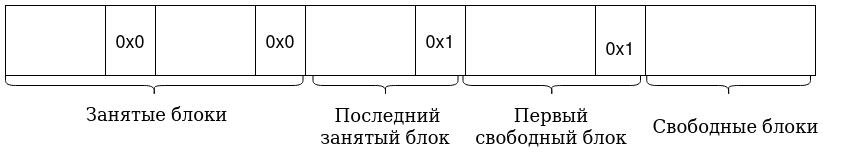
\includegraphics[width=\linewidth]{allocation_in_progress.png}
    \end{figure}
    
    \begin{figure}[H]
      \centering
      \caption{Структура кучи NVRAM после перемещения границы аллокации вправо}
      \label{allocation-finished-pic}
      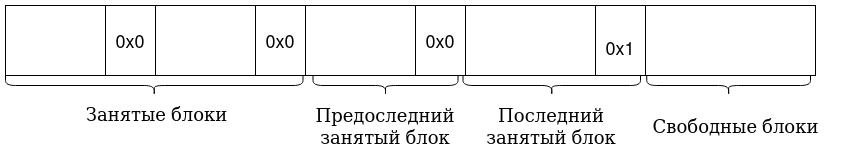
\includegraphics[width=\linewidth]{allocation_finished.png}
    \end{figure}
\end{itemize}

\section{Второй алгоритм: освобождение памяти}

Если алгоритму приходит запрос на освобождение блока памяти, возможны два варианта:

\begin{itemize}
    \item Блок памяти, который требуется освободить, не является самым правым выделенным блоком. В таком случае в $(k + 1)$-ом байте этого блока записано \texttt{0x0}. Тогда просто запишем в $(k + 1)$-ый байт этого блока \texttt{0x2} и добавим этот блок в множество свободных.
    
    \item Блок памяти, который требуется освободить, является самым правым выделенным блоком (см. Рисунок \ref{before-free-pic}). В таком случае необходимо переместить влево границу аллокации. Для этого необходимо найти самый правый выделеный блок, не совпадающий с блоком, который необходимо освободить (это будет самый правый блок, в $(k + 1)$-ом байте которого записано \texttt{0x0}). Этот блок и станет новой границей аллокации, необходимо записать \texttt{0x1} в его $(k + 1)$-ый байт. Очевидно, между новой и старой границей аллокации могут быть несколько свободных блоков (в $(k + 1)$-ом байте этих блоков записано \texttt{0x2}). После перемещения границы аллокации влево эти блоки окажутся справа от границы аллокации, поэтому их необходимо удалить из множества свободных блоков (см. Рисунок \ref{after-free-pic}).  
    
    \begin{figure}[H]
      \centering
      \caption{Структура кучи NVRAM до перемещения границы аллокации влево}
      \label{before-free-pic}
      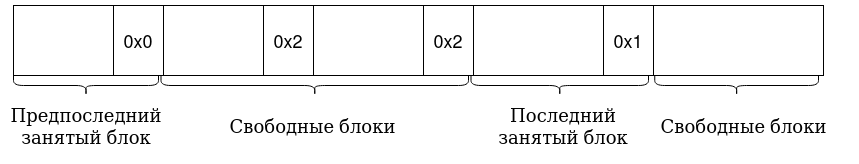
\includegraphics[width=\linewidth]{before_free.png}
    \end{figure}
    
    \begin{figure}[H]
      \centering
      \caption{Структура кучи NVRAM после перемещения границы аллокации влево}
      \label{after-free-pic}
      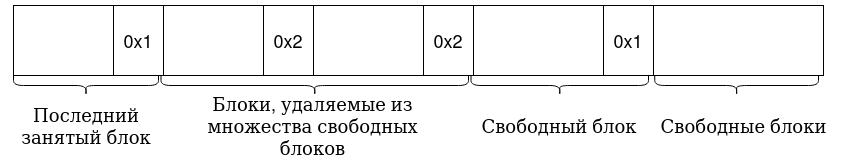
\includegraphics[width=\linewidth]{after_free.png}
    \end{figure}
\end{itemize}

\section{Второй алгоритм: сбои системы}

Заметим, что вышеописанный алгоритм требует гарантии атомарности записи всего одного байта, поэтому его можно использовать на системах, использующих жёсткие диски в качестве энергонезависимого хранилища. Куча NVRAM никогда не будет приведена в неконсистентное состояние из-за того, что сбой системы произошёл в процессе записи.

Если произойдёт сбой системы, состояние аллокатора (граница аллокации и список свободных блоков), хранившееся в энергозависимой памяти, будет потеряно. Чтобы восстановить его, необходимо после запуска системы пройти по куче NVRAM от начала до первого блока, у которого в $(k + 1)$-ом байте записано \texttt{0x1}. Порядковый номер этого блока станет границей аллокации, а порядковые номера всех встреченных в процессе обхода блоков, у которых в $(k + 1)$-ом байте записано \texttt{0x2}, сформируют множество свободных блоков.

Кроме того, сбой системы может привести к утечке памяти. Представим, например, ситуацию, когда некий блок в куче NVRAM был помечен как выделенный (например, мы изменили значение его $(k + 1)$-ого байта с \texttt{0x2} на \texttt{0x0}), и в этот момент произошёл сбой системы (до того, как мы успели вернуть вызывающей стороне адрес выделенного блока). Для борьбы с этим можно применить подход, описанный в работе \cite{cai2020understanding}. Этот подход заключается в запуске процедуры сборки мусора после возобновления работы системы, которая позволяет разметить недоступные, но не освобождёные, блоки памяти. После разметки таких блоков эти блоки можно освободить.

\section{Выбор используемого для реализации системы алгоритма}

В работе нам необходимо эмулировать NVRAM на системах, использующих жёсткие диски в качестве энергонезависимого хранилища. Эти системы могут не предоставлять гарантию атомарности записи в энергонезависимое хранилище восьми байт, выровненных по размеру кэш-линии, но предоставляют гарантию атомарности записи одного байта. Следовательно, при использовании первого алгоритма, куча NVRAM может прийти в неконсистентное состояние, если произойдёт сбой в процессе записи восьми байт, определяющих границу аллокации в первом алгоритме.

Кроме того, заметим, что ограничение второго алгоритма (возможность выделять только блоки памяти фиксированного размера) не является существенным ограничением при реализации системы, так как выделение динамической памяти в куче NVRAM используется только под ответ задачи \texttt{CAS} фиксированного размера (по одному байту на каждый ответ).

Следовательно, при реализации системы будет использоваться второй алгоритм выделения памяти в куче NVRAM.

\chapterconclusion

В этой главе была рассмотрена задача выделения памяти в куче NVRAM и разработаны два алгоритма выделения памяти. Первый алгоритм допускает выделение блоков памяти произвольного размера, но не поддерживает освобождение выделенной памяти и требует для работы гарантии атомарности записи восьми байт, выровненных по размеру кэш-линии. Второй алгорим поддерживает выделение блоков памяти только фиксированного размера, зато этот алгоритм поддерживает особождение выделенной памяти и требует для корректной работы гарантию атомарности записи только одного байта.

В силу специфики работы, при реализации системы будет использоваться второй алгоритм.

\chapter{Практическое применение}

\section{CAS для NVRAM}

Алгоритм \texttt{CAS} для NVRAM, удовлетворяющий условию корректности Nesting-safe recoverable linearizability, описан в статье \cite{attiya2018nesting}.

В статье предполагается отсутствие энергозависимых кэшей у NVRAM, поэтому после каждой записи в NVRAM будем немедленно производить сброс кэшей чтобы записанные данные попали в NVRAM немедленно после записи.

Для корректности описанного в статье алгоритма требуется, чтобы каждая запись в NVRAM выполнялась атомарно. Так как атомарно в NVRAM можно сбросить только одну кэш-линию, потребуем чтобы ни одна запись не пересекала границ кэш-линии.

В ходе исполнения алгоритма запись может быть произведена только в \texttt{C}~--- RMW-регистр, по которому делается CAS и в $R_{i, j}$~--- один из single-reader-single-writer (SRSW) регистров из квадратной марицы \texttt{R}. $R_{i, j}$ используется потоком $t_j$ для того, чтобы уведомить поток $t_i$ о том, что осуществлённый потоком $t_i$ \texttt{CAS} был успешен.

Пусть адрес начала \texttt{C} выровнен по размеру кэш-линии, сам RMW-регистр \texttt{C} занимает восемь байт. В таком случае, регистр \texttt{C} целиком помещается в единственной кэш-линии архитектуры x86, не пересекая её границ (так как в архитектуре \texttt{x86} кэш-линии имеют размер 64 байта). Таким образом, запись RMW-регистра \texttt{C} приводит к сбросу в NVRAM всего одной кэш-линии, и, следовательно, выполняется атомарно.

Пусть матрица \texttt{R} хранится по строкам, то есть сначала в памяти уложена первая строка матрицы, потом вторая, потом третья, и так до \texttt{N}-ой (см. Рисунок \ref{r-matrix-pic}).

\begin{figure}[H]
  \centering
  \caption{Расположение матрицы SRSW-регистров в NVRAM}
  \label{r-matrix-pic}
  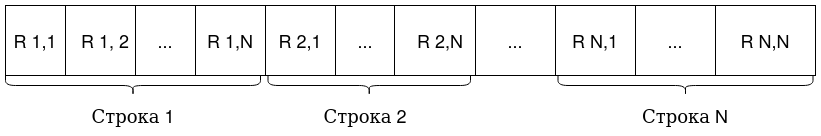
\includegraphics[width=\linewidth]{matrix.png}
\end{figure}

Если каждый из SRWR регистров $R_{i, j}$ занимает четыре байта, а начало матрицы выровнено по размеру кэш-линии, то ни один из регистров не пересекает кэш-линию ни при каком значении $N$. Таким образом, запись в любой из SRSW-регистров $R_{i, j}$ приводит к сбросу в NVRAM всего одной кэш-линии, а значит, выполняется атомарно.

\section{Задача тестирования CAS}

Рассмотрим последовательность операций $\{CAS(var, expected_j, new_j)\}_{j = 1}^M$, исполняемых потоками $\{t_i\}_{i = 1}^N$.  Заметим, в частности, что все операции выполняются на одном регистре.

Рассмотрим, кроме того, бинарное отношение happens before на этих операциях. Это отношение подробно описано, например, в статье \cite{lamport2019time}. Если операции $a$ и $b$ связаны этим отношением в исполнении $H$, будем обозначать это $HB_H(a, b)$ или $a \rightarrow_H b$.

Пусть мы хотим проверять исполнение операций $\{CAS(var, expected_i, new_i)\}_{j = 1}^M$ на линеаризуемость.

Назовём исполнение $H$ линеаризуемым, если оно эквивалентно какому-то последовательному исполнению $L$, при этом из $a \rightarrow_H b$, должно следовать $a \rightarrow_L b$. Более подробно данное условие корректности рассмотрено в статье \cite{herlihy1990linearizability}.

Так как проверка исполнения на линеаризуемость в некоторых случаях является слишком сложной задачей, рассмотрим также сериализуемость~--- более слабое условие корректности в многопоточной среде. Назовём исполнение $H$ сериализуемым, если оно эквивалентно какому-то последовательному исполнению $L$. Заметим, что из $a \rightarrow_H b$ может не следовать $a \rightarrow_L b$. Более подробно это условие корректности рассмотрено в статье \cite{papadimitriou1979serializability}. 

Применим разработанный в предыдущих главах алгоритм запуска программ для NVRAM для проверки на сериализуемость и линеаризуемость алгоритма CAS, описанного в статье \cite{attiya2018nesting}. 

В дальнейшем будем называть $init$ начальное значение RMW-регистра, по которому делается CAS (то есть то значение, которое было записано в регистре до выполнения любой из операции).

\section{Тестирование CAS с ограничениями}
\label{restricted-cas-checking}
Для того, чтобы проверить исполнение на линеаризуемость, введём на операции несколько дополнительных ограничений.

\begin{itemize}
    \item Каждое значение $new_j$ из $\{\{CAS(var, expected_j, new_j)\}_{j = 1}^{M}$ должно быть уникальным, то есть для любого значения $a$ можно найти не более одного такого $j$, что $new_j = a$.
    
    \item Для всех $j: new_j \ne init$, то есть ни одно значение $new_j$ из $\{\{CAS(var, expected_j, new_j)\}_{j = 1}^{M}$ не должно совпадать с исходным значением переменной. Это условие, вкупе с предыдущим, утверждает, что каждое значение, включая исходное, могло оказаться в переменной не более чем единожды.
    
    \item  Для всех $j: new_j \ne expected_j$.
\end{itemize}

\bigbreak

Если последовательность операций удовлетворяет таким ограничениям, то исполнение можно проверять на линеаризуемость.

Для проверки исполнения на линеаризуемость построим ориентированный граф $G = \langle V, E \rangle$, при этом множество вершин графа имеет вид $V = \{new_j\}_{j = 1}^M \cup \{expected_j\}_{j = 1}^M \cup init$. Множество рёбер $E$ строится следующим образом: между вершинами $a$ и $b$ есть ребро $a \rightarrow b$, если среди исполненых операций был успешный $CAS(var, a, b)$ (то есть существует $j$, такое что $expected_j = a$ и $new_j = b$, и при этом $CAS(var, expected_j, new_j)$ был успешен).

Построенный граф имеет следующие свойства:


\begin{itemize}
    \item Из того, что $new_j \ne expected_j$, следует, что в графе не может быть петель. 
    
    \item В вершину, соответствующую начальному значению, не может входить ни одно ребро, так как $\forall j: new_j \ne init$. Следовательно, ни для какого $a$ в исполнении не могло найтись успешного $CAS(var, a, init)$.
    
    \item Ни в одну вершину не может войти больше одного ребра. Пусть это не так и найдутся три такие вершины $(a, b, c)$, что $a \rightarrow b, c \rightarrow b$. Это значит, что в исполнении был успешный $CAS(var, a, b)$ и успешный $CAS(var, c, b)$. Значит,  $new_j$ не уникальны, так как как минимум в двух различных операциях  $new_j = b$. 
\end{itemize}

\bigbreak

Заметим, что если в этом графе найдутся три такие различные вершины $(a, b, c)$, что $a \rightarrow b, a \rightarrow c$ (см. Рисунок \ref{incorrect-graph-pic}), то такое исполнение нелинеаризуемо. Действительно, так как значение переменной $var$ не могло одновременно смениться с $a$ и на $b$, и на $c$, такое могло произойти только в одном случае:

\begin{itemize}
    \item Пусть в какой-то момент в переменной было записано значение $a$.
    
    \item Потом в исполнении случился успешный $CAS(var, a, b)$, в результате которого значение сменилось на $b$, или успешный $CAS(var, a, c)$, в результате которого значение сменилось на $c$. В силу симметричности этих случаев предположим, что произошёл успешный $CAS(var, a, b)$ и значение сменилось с $a$ на $b$, а в графе появилось ребро $a \rightarrow b$.
    
    \item Потом значение снова сменилось на $a$.
    
    \item Потом произошёл успешный $CAS(var, a, c)$, в результате которого значение сменилось с $a$ на $c$, а в графе появилось ребро $a \rightarrow c$.
\end{itemize}

\bigbreak

Заметим, что в таком случае значение $a$ оказалось записано в переменную более чем единожды, а по условиям такого быть не может.

\begin{figure}[H]
  \centering
  \caption{Пример графа, соответствующего не линеаризуемому исполнению}
  \label{incorrect-graph-pic}
  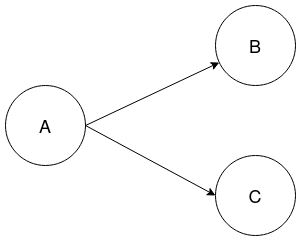
\includegraphics[width=\linewidth]{incorrect_graph.png}
\end{figure}

Теперь заметим, что если в графе нашлись такие вершины $a, b$ что $a \rightarrow b$, при этом $a \ne init$ и не существует $c$ с $c \rightarrow a$ (см. Рисунок \ref{incorrect-graph-2-pic}), то такое исполнение не линеаризуемо. 

Действительно, исходное значение переменной не было равно $a$ и в исполнении не было успешной операции $CAS(var, c, a)$. Таким образом, значение переменной ни в какой момент не могло стать равным $a$, значит, ни для какого значения $b$ операция $CAS(var, a, b)$ не могла закончиться успешно, таким образом, в графе не может существовать ребра $a \rightarrow b$.

\begin{figure}[H]
  \centering
  \caption{Пример графа, соответствующего нелинеаризуемому исполнению}
  \label{incorrect-graph-2-pic}
  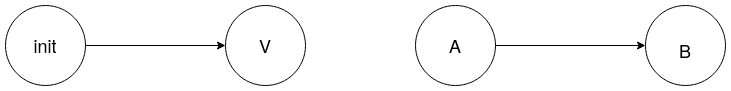
\includegraphics[width=\linewidth]{incorrect_graph_2.png}
\end{figure}

Из этого следует, что линеаризуемому исполнению соответствует только один вид графов (см. Рисунок \ref{correct-graph-pic}): те, в которых рёбра образуют единственный эйлеров путь, начинающийся в вершине, соответствующей начальному значению и заканчивающийся в вершине, соответствующей значению регистра $var$ после исполнения всех операций (то есть граф является ``бамбуком''). Если такой путь найти не удаётся, то исполнение точно не линеаризуемо.

\begin{figure}[H]
  \centering
  \caption{Пример графа, возможно соответствующего линеаризуемому исполнению}
  \label{correct-graph-pic}
  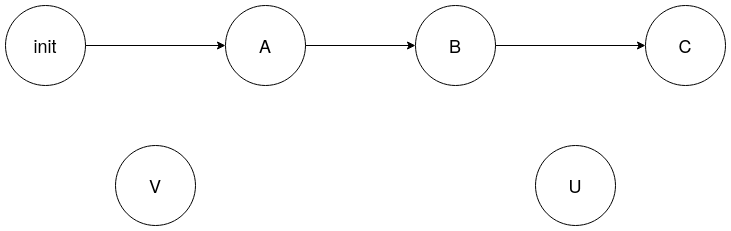
\includegraphics[width=\linewidth]{correct_graph.png}
\end{figure}

Если же удалось найти такой путь, то нам удалось найти единственное возможное последовательное исполнение $L$, эквивалентное исполнению $H$. При этом не может существовать другое последовательное исполнение $L'$, эквивалентное данному, так как в графе существует единственный эйлеров путь.

Для завершения проверки линеаризуемости остаётся только проверить, исполнение $L$ учитывает ограничения, заданные отношением happens-before (то есть $a \rightarrow_H b \Rightarrow a \rightarrow_L b$). 

Заметим, что исполнение $L$ последовательное, поэтому оно задаёт полный порядок на операциях. Поэтому для того, чтобы проверить, что отношение $L$ удовлетворяет ограничениям happens-before нужно для каждой пары операций \begin{equation*}
CAS(var, a, b), CAS(var, c, d):
 \begin{cases}
   CAS(var, a, b) \rightarrow_H CAS(var, c, d)\\
   CAS(var, a, b) = true \\
   CAS(var, c, d) = true
 \end{cases}
\end{equation*} проверить, что ребро $a \rightarrow b$ в найденном эйлеровом пути идёт до ребра $c \rightarrow d$.  Еси это верно, то исполнение $H$ линеаризуемо. Если же это неверно, то исполнение $H$ не линеаризуемо, но сериализуемо (так как существует последовательное исполнение $L$, эквивалентное исполнению $H$, но не существует последовательного исполнения $L'$, эквивалентного исполнению $H$ и учитывающего ограничения, заданные отношением happens-before).

\section{Тестирование CAS}

Можно отказаться от ограничений, введённых в начале предыдущего пункта, и проверять на сериализуемость исполнение произвольной последовательности $\{CAS(var, expected_j, new_j)\}_{j = 1}^M$.

Построим ориентированный граф $G = \langle V, E \rangle$ по тем же принципам, что и в предыдущем пункте. В этот раз из-за отсутствия наложенных в предыдущем пункте ограничений в графе могут быть:

\begin{itemize}
    \item Петли, так как разрешены операции вида $CAS(var, a, a)$
    
    \item Такие тройки различных вершин $(a, b, c)$, что $a \rightarrow b, a \rightarrow c$, так как значение $а$ могло быть записано в переменную больше одного раза.
    
    \item Такие тройки различных вершин $(a, b, c)$, что $a \rightarrow b, c \rightarrow b$, так как нет ограничения на уникальность $new_j$ и можно найти более одного такого $j$, что $new_j = b$.
    
    \item Более одного ребра $a \rightarrow b$, так как в исполнении могло быть более одной успешной операции $CAS(var, a, b)$.
\end{itemize}

\bigbreak

Теперь для того, чтобы проверить сериализуемость исполнения, необходимо найти произвольное последовательное исполнение, эквивалентное полученному, при этом найденное последовательное исполнение может не учитывать ограничения, заданные отношением happens-before.

Рассмотрим произвольный путь, проходящий по графу $G$. Каждое ребро $a \rightarrow b \in E$ сответствует исполнению одной операции $CAS(var, a, b)$. Так как каждый успешный CAS был исполнен ровно один раз, нужно найти такой путь в графе, который проходит по каждому ребру ровно один раз, то есть найти эйлеров путь. При этом известно, что начальное значение регистра $var$ было равно $init$, а значит найденный эйлеров путь должен начинаться в вершине, соответствующей значению $init$. При этом нам так же известно значение $finish$~--- значение регистра $var$ после исполнения всех операций. Значит, найденный эйлеров путь должен заканчиваться в вершине, соответствующей значению $finish$.

В таком случае проверка исполнения на сериализуемость сводится к нахождению эйлерова пути, начинающегося в вершине, соответствующей значению $init$ и заканчивающегося в вершине, соответствующей значению $finish$.

Для проверки на сериализуемость используем следующий алгоритм:

\begin{itemize}
    \item Если более одной компоненты слабой связности содержат хотя бы одно ребро, то исполнение несериализуемо, так как в таком случае в графе не существует ни одного эйлерова пути.

    \item Для каждой вершины $v$ считаем количество входящих в неё и исходящих из неё рёбер $deg^+(v), deg^-(v)$.
    
    \item Если $deg^+(v) = deg^-(v)$ для любого $v \in V$, в графе существует эйлеров цикл. Если вершина, соответствующая значению $init$, входит в этот цикл и при этом $init = finish$, значит, исполнение сериализуемо ~--- выберем эйлеров путь таким образом, чтобы он начинался и заканчивался в вершине, соответствующей значению $init$. В противном случае исполнение не сериализуемо. 
    
    \item Если  для любого $v \in V \setminus \{a, b\}: deg^+(v) = deg^-(v),$
    $deg^+(a) = deg^-(a) - 1,  deg^+(b) = deg^-(b) + 1$, то исполнение сериализуемо только в том случае, если вершина $a$ соответствует значению $init$, а вершина $b$ соответствует значению $finish$ (так как найденный эйлеров путь может начинаться только в вершине $a$, а заканчиваться только в вершине $b$).
\end{itemize}

\section{Характеристики и результаты тестирования}

Тестирование алгоритма \texttt{CAS} для NVRAM происходило в следующем окружении:

\begin{itemize}
    \item Для тестирования использовалось четыре рабочих потока.
    
    \item NVRAM эмулировалась с помощью файлов, отображаемых в память. В качестве энергонезависимого хранилища использовались жёсткие диски. Для сброса кэша из оперативной памяти в энергонезависимое хранилище использовался системный вызов \texttt{msync} \cite{msync}.
    
    \item Сбой системы эмулировался с помощью посылания сигнала \texttt{SIGKILL} всему процессу (то есть прерывался главный поток и все рабочие потоки). Для посылки процессу сигнала \texttt{SIGKILL} использовалась утилита \texttt{kill} \cite{kill}.
    
    \item Для того, чтобы операцию \texttt{CAS} можно было успеть прервать в процессе её выполнения (и таким образом проверить, что даже сбой системы в процессе выполнения операции не нарушает линеаризуемости исполнения), в код операции \texttt{CAS} было помещено несколько инструкций \texttt{sleep}, позволяющих замедлить выполнение операции. 
\end{itemize}

\bigbreak

Алгоритм \texttt{CAS} из статьи \cite{attiya2018nesting} был проверен на нескольких десятках сценариев, при этом учитывались ограничения из секции \ref{restricted-cas-checking}. Каждое из полученных в ходе тестирования исполнений оказалось линеаризуемо.

\section{Тестирование некорректного алгоритма CAS}

Рассмотрим некорректный алгоритм \texttt{CAS} для NVRAM, в котором отсутствует матрица \texttt{R}, обеспечивающая связь между читателями и писателями. Считаем, что \texttt{Var} - 32х-битный регистр, расположенный в NVRAM. Псевдокод этого алгоритма может выглядеть следующим образом (см. Листинг \ref{incorrect-cas-algorithm}): 

\begin{algorithm}[H]
\caption{Псевдокод некорректного алгоритма CAS}
\label{incorrect-cas-algorithm}
\begin{algorithmic}
    \Function{cas\_incorrect}{$Var, expected, new$}
        \State result = CAS(Var, expected, new)
        \If{result} 
            \State pmem\_flush(Var, 4)
            \State \Return true 
        \Else 
            \State \Return false
        \EndIf
    \EndFunction
    
    \bigbreak
    \bigbreak
    
    \Function{cas\_incorrect\_recover}{$Var, expected, new$}
        \State uint32\_t cur\_value
        \State pmem\_read(Var, \&cur\_value, 4)
        \If{cur\_value == new}
            \State \Return true 
        \Else 
            \State \Return cas\_inocrrect(Var, expected, new)
        \EndIf
    \EndFunction
\end{algorithmic}
\end{algorithm}

Рассмотрим следующее исполнение, нескольких операций \texttt{CAS} двумя потоками (\texttt{A} и \texttt{B}).

\begin{itemize}
    \item Пусть изначальное значение переменной равно 42
    \item Поток \texttt{A} исполняет \texttt{CAS(Var, 42, 24)}.
    \item Одновременно поток \texttt{B} исполняет \texttt{CAS(Var, 24, 14)}.
    \item Поток \texttt{A} успешно завершает свою операцию (значение переменной меняется с 42 на 24), но засыпает, не вернув \texttt{true} вызывающей стороне.
    \item Поток \texttt{B} успешно завершает свою операцию (значение переменной меняется с 24 на 14) и возвращает значение. \texttt{true} вызывающей стороне
    \item В этот момент происходит сбой системы
    \item После сбоя системы в потоке \texttt{A} вызывается операция \texttt{cas\_incorrect\_recover(Var, 42, 24)}, возвращающая \texttt{false} (так как текущее значение переменной \texttt{Var} равно 14).
\end{itemize}

\bigbreak

Таким образом, соответствующий исполнению граф выглядит следующим образом
(см. Рисунок~\ref{incorrect-cas-pic}):

\begin{figure}[H]
  \centering
  \caption{Граф, соответствующий исполнению}
  \label{incorrect-cas-pic}
  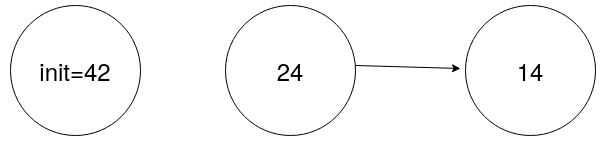
\includegraphics[width=\linewidth]{incorrect_cas_graph.png}
\end{figure}

Как показано в секции \ref{restricted-cas-checking}, это исполнение не линеаризуемо. Потребовалось три запуска разработанной мной системы, чтобы обнаружить нелинеаризуемое исполнение некорректного алгоритма \texttt{CAS} для NVRAM.

\chapterconclusion

В этой главе было рассмотрено применение разработанного алгоритма для тестирования алгоритма \texttt{CAS} для NVRAM. Рассмотрены два метода проверки алгоритма \texttt{CAS} для NVRAM на корректность: с помощью первого метода можно проверить исполнение \texttt{CAS} с ограничениями на линеаризуемость, а с помощью второго метода можно проверить исполнение \texttt{CAS} без ограничений на сериализуемость. Кроме того, в этой главе был описан процесс тестирования алгоритма \texttt{CAS} для NVRAM, описанного в статье \cite{attiya2018nesting}, и тестрования некорректного алгоритма \texttt{CAS} для NVRAM.

%% Макрос для заключения. Совместим со старым стилевиком.
\startconclusionpage

Мне удалось разработать алгоритм запуска программ для NVRAM, который запускает программы в модели Nesting-safe recoverable linearizability и восстанавливает систему после сбоя. Этот алгоритм удалось проэмулировать без доступа к NVRAM, с использованием только жёстких дисков. Следовательно, разработанный алгоритм можно  использовать как для запуска программ в системе с использованием NVRAM, так и в системе с использованием жёстких дисков в качестве энергонезависимого хранилища. Например, разработаный алгоритм можно использовать для тестирования алгоритмов для NVRAM без доступа к железу с NVRAM.

Кроме того, мне удалось протестировать алгоритм \texttt{CAS} для NVRAM на корректность, используя разработанную мной систему.

\bigbreak

Можно предложить несколько путей развития и улучшения существующего решения. Например, можно выполнять следующие преобразования пользовательского кода:

\begin{itemize}
    \item Автоматически выполнять сериализацию/десериализацию параметров функции в массив байт и из массива байт, позволяя пользователю принимать и передавать аргументы привычным способом.
    
    \item Автоматически регистрировать все необходимые функции в глобальной хеш-таблице.
    
    \item Позволить пользователю вызывать функцию привычным образом, а не через \texttt{do\_call}, автоматически вставляя код для добавления нового фрейма и перемещения конца стека.
    
    \item Автоматически вставлять код для сохранения возвращаемого значения.
    
    \item Автоматически вставлять код для преобразования указателей на NVRAM в смещения от начала отображения NVRAM в виртуальное адресное пространство.
\end{itemize}

\printmainbibliography

%% После этой команды chapter будет генерировать приложения, нумерованные русскими буквами.
%% \startappendices из старого стилевика будет делать то же самое
\appendix

\end{document}